\documentclass{sysuthesis} % xiaosi == 12pt
%---- whether double spacing
%\usepackage{setspace}
%----

%\usepackage{scrhack} %消除listings包产生的警告信息
%----展现代码
%\usepackage{listings}
%\lstset{language=C}
%----
%----Set the theorems 定理环境


\usepackage{color}
\usepackage{amsmath}
\usepackage{amssymb} %for $\diagdown \llap{a}$
\usepackage{amsthm}
\usepackage{algorithm}
\usepackage{algpseudocode}
%\usepackage{enumitem}
\usepackage{listings}
\usepackage{setspace}
\numberwithin{algorithm}{chapter}
\floatname{algorithm}{算法}
\renewcommand{\algorithmicforall}{\textbf{for each}}
\newcolumntype{C}[1]{>{\centering\let\newline\\\arraybackslash\hspace{0pt}}m{#1}}
\renewcommand{\arraystretch}{1.3}
\renewcommand{\algorithmicrequire}{ \textbf{输入:}} %Use Input in the format of Algorithm  
\renewcommand{\algorithmicensure}{ \textbf{输出:}} %UseOutput in the format of Algorithm 


%\usepackage{footmisc}


\usepackage{threeparttable}

%得益于amsthm,我们可以定义不同环境的样式
\theoremstyle{plain}
\newtheorem{assumption}{假设}[chapter]
\newtheorem{proposition}{命题}[chapter]
\newtheorem{lemma}{引理}[chapter]
\newtheorem{theorem}{定理}[chapter] %按章编号
\newtheorem{axiom}{公理}[chapter]
\newtheorem{corollary}{推论}[chapter]

\theoremstyle{definition}
\newtheorem{definition}{定义}[chapter]
\newtheorem{exercise}{练习}[chapter]
\newtheorem{example}{例}[chapter]

\theoremstyle{definition}
\newtheorem{remark}{注释}[chapter]
\newtheorem{problem}{问题}[chapter]
\newtheorem{conjecture}{猜想}[chapter]




\setlength{\footskip}{25pt}

%\newtheorem{exercise}{Exercise}
%\newtheorem{suppexercise}[exercise]{Supplementary Exercise}%编号依赖前一个环境,与环境exercise共用一个计数器

%得益于amsthm,所以
%\newtheorem*{note}{Note} %不参与计数
%----ff

%----Algorithm
%\usepackage[algo2e]{algorithm2e}
%----

%----打印数字和一些符号的包
%\usepackage{siunitx}
%----

\usepackage{fancyvrb} % 带框的Verbatim,不是verbatim

%----back reference the citation
%    最好放在所以包的最后
%\usepackage[]{hyperref}
%\usepackage[backref]{hyperref}
%----
%\includeonly{method,results} % only work one these two chapter

% 定义所有的eps文件在 figures 子目录下
\graphicspath{{figures/}}

\newcommand{\ignore}[1]{{}}
\newcommand{\mylist}[1]{
	\begin{spacing}{2.5}
	\noindent\textbf{* {#1}}
	\end{spacing}
}

%\newcommand{\f}[1]{{\color{red}#1}}



\begin{document}
\title{基于增量图表征的属性网络研究}{}{Attributed Network Analysis via Incremental Network Embedding}{}

%\author{李友}{You Li}
%\advisor{郑子彬}{副教授}{Zibin Zheng}{Associate Professor}
%\major{计算机技术}{Computer Technology}
%\school{数据科学与计算机学院}
\author{}{}
\advisor{}{}{}{}
\major{}{}
\school{}


\finishdate{二零一八 \hspace{1mm}年\hspace{3mm}五\hspace{3mm}月} %答辩日期

%\thanks{感谢国家自然科学基金 (编号为xxxxx)的支持。}

\maketitle

\begin{abstract}{属性网络,增量学习,图表征,矩阵分解,降维学习}
  随着社交网络的发展,网络数据的规模越来越庞大。海量的网络型数据对服务提供者包含着前所未有的机遇和挑战。对于服务提供者而言,可以利用对海量网络型数据的挖掘指导业务发展,如社交网络中通过网络的挖掘研究,可以进行高效的好友推荐;金融服务可以通过有效的挖掘任务规避用户在包括信用卡,借贷等信用业务中逾期甚至欺诈的风险。在机遇的同时,海量的网络型数据更带来巨大的挑战:一方面,对于海量的网络型数据直接进行数据处理和分析存储和计算成本非常巨大;另一方面,真实的网络数据是处在一直演化变动的过程中的,每当新增节点或连边就重新进行网络挖掘任务成本更是非常巨大。因此在网络挖掘中如何进行有效的网络信息抽取是一个非常值得研究的课题。在海量数据处理研究方面,用来提取数据重要信息的手段被称之为数据降维。受数据降维的启发,网络挖掘领域的图表征算法在近几年研究领域中引起非常大的关注。

本文的研究对象是现实场景中最常见的属性网络,也即网络中的节点除了网络连接结构以外,也包含大量的节点特征,例如社交网络中用户节点包含丰富的属性信息:账号、年龄、兴趣爱好等,对于节点属性的利用将更有利于网络型数据的学习任务。同时,属性网络的另一个特点也是本文的研究内容,即网络的动态演化。本文就动态演化的属性网络进行挖掘任务,对于网络结构提出一种新的算法进行网络表征,通过相似度计算保留网络结构上的高阶接近度,也即保留网络中大于一度邻居的局部信息;基于这个算法提出相应的增量表征算法来处理动态场景下的网络表征;对于节点属性提出一种新的算法进行属性降维学习,节点属性不同于网络结构的稀疏性,提出适合梯度下降的方式进行数据降维;同时提出相应的增量降维学习算法对动态网络。

实验结果表明,本文提出的网络表征方式和增量表征方式在后续的节点分类任务中都表现出理想的准确率和不错的时间效率。
\end{abstract}

\begin{englishabstract}{Attributed network, Incremental learning, Network embedding, Matrix Factorization, dimensionality reduction}
  With the development of social networks, the scale of network data is increasing. The massive network data contains unprecedented opportunities and challenges for service providers. For service providers, they can use the data mining of large amounts of network data to guide business development. For example, through social network mining research, high-performance friend recommendation can be performed; financial services  can evade the risk of overdue or even fraud in credit transactions  through effective mining tasks. At the same time, massive network-based data poses enormous challenges. On the one hand, data processing and analysis for huge amounts of network-based data are very costly in storage and calculation; on the other hand, the real-world network data is in the process of evolution,  restarting network mining tasks is very costly whenever new nodes or edges are modified. Therefore, how to extract effective network information in network mining is a very worthy research topic. In the research of massive data processing, the method used to extract important information from the data is called data dimensionality reduction. Inspired by data dimensionality reduction, network embedding algorithms have attracted much attention in research in recent years.

The research object of this paper is the most common attribute network in the real scene. That is to say, the nodes in the network have a lot of node features in addition to the network connection structure. For example, the user nodes in the social network contain rich attribute information: account number, age, interest,  etc., the use of node attributes will be more advantageous to the learning task of network data. At the same time, another characteristic of attribute network is the research content of this paper, namely the dynamic evolution of the network. In this paper, a new network embedding algorithm based on Laplacian Eigenmaps for the network structure is proposed , and similarity calculation is used to preserve the high-order proximity of the network structure, that is, to retain the local information in the network that is greater than the first-degree neighbor. Based on this algorithm, a corresponding incremental network embedding algorithm is proposed to deal with the dynamic network. A new algorithm is proposed for node attributes to perform representation learning. The node attributes are different from the sparsity of the network structure and a method suitable for gradient descent is proposed.  At the same time, a corresponding incremental attributes representation learning algorithm is proposed for dynamic networks.

In this paper, experimental results show that the network representation and incremental representation have ideal accuracy and good time efficiency in subsequent node classification and link prediction tasks.

\end{englishabstract}

\tableofcontents
%\listoffigures
%\listoftables

%\begin{terminology}
%  本论文专用术语的注释表
%\end{terminology}

\begin{Main} % 开始正文
\chapter{绪论}

%%%%%%%%%%%%%%%%%%%%%%%%%%%%%%%%%%%%%%%
%-----------------------------------     研究背景和意义     -----------------------------------%
%%%%%%%%%%%%%%%%%%%%%%%%%%%%%%%%%%%%%%%
本章内容主要介绍论文的研究背景和意义、研究现状、论文的工作与创新点和论文的组织结构
\section{研究背景和意义}
在飞速发展的互联网影响下,越来越多的网络数据积累下来。网络结构数据涉及的领域也越来越广,不同领域的应用都少不了对网络类数据的挖掘,比如社交网络、通信网络、生物蛋白质网络,金融交易网络,这些网络都是用来表示一个个复杂系统,在网络中,节点用来表示复杂系统的个体或实体,连边表示个体或实体间的相互关系,比如社交网络中的相互关注、互为好友,通信网络中的相互连接,生物蛋白质之间的相互作用等。随着覆盖领域的扩大,越来越多的现实应用需要挖掘网络中的信息,比如社交网络Twitter\footnote{www.twitter.com}的推荐系统需要通过挖掘网络信息而实现给用户推荐符合用户偏好的推文,广告精准投放系统中通常需要将社交网络中的用户分成不同的社区来提高精度。因此,挖掘网络中的信息是非常具有实际价值的。

\begin{figure}
	\centering
	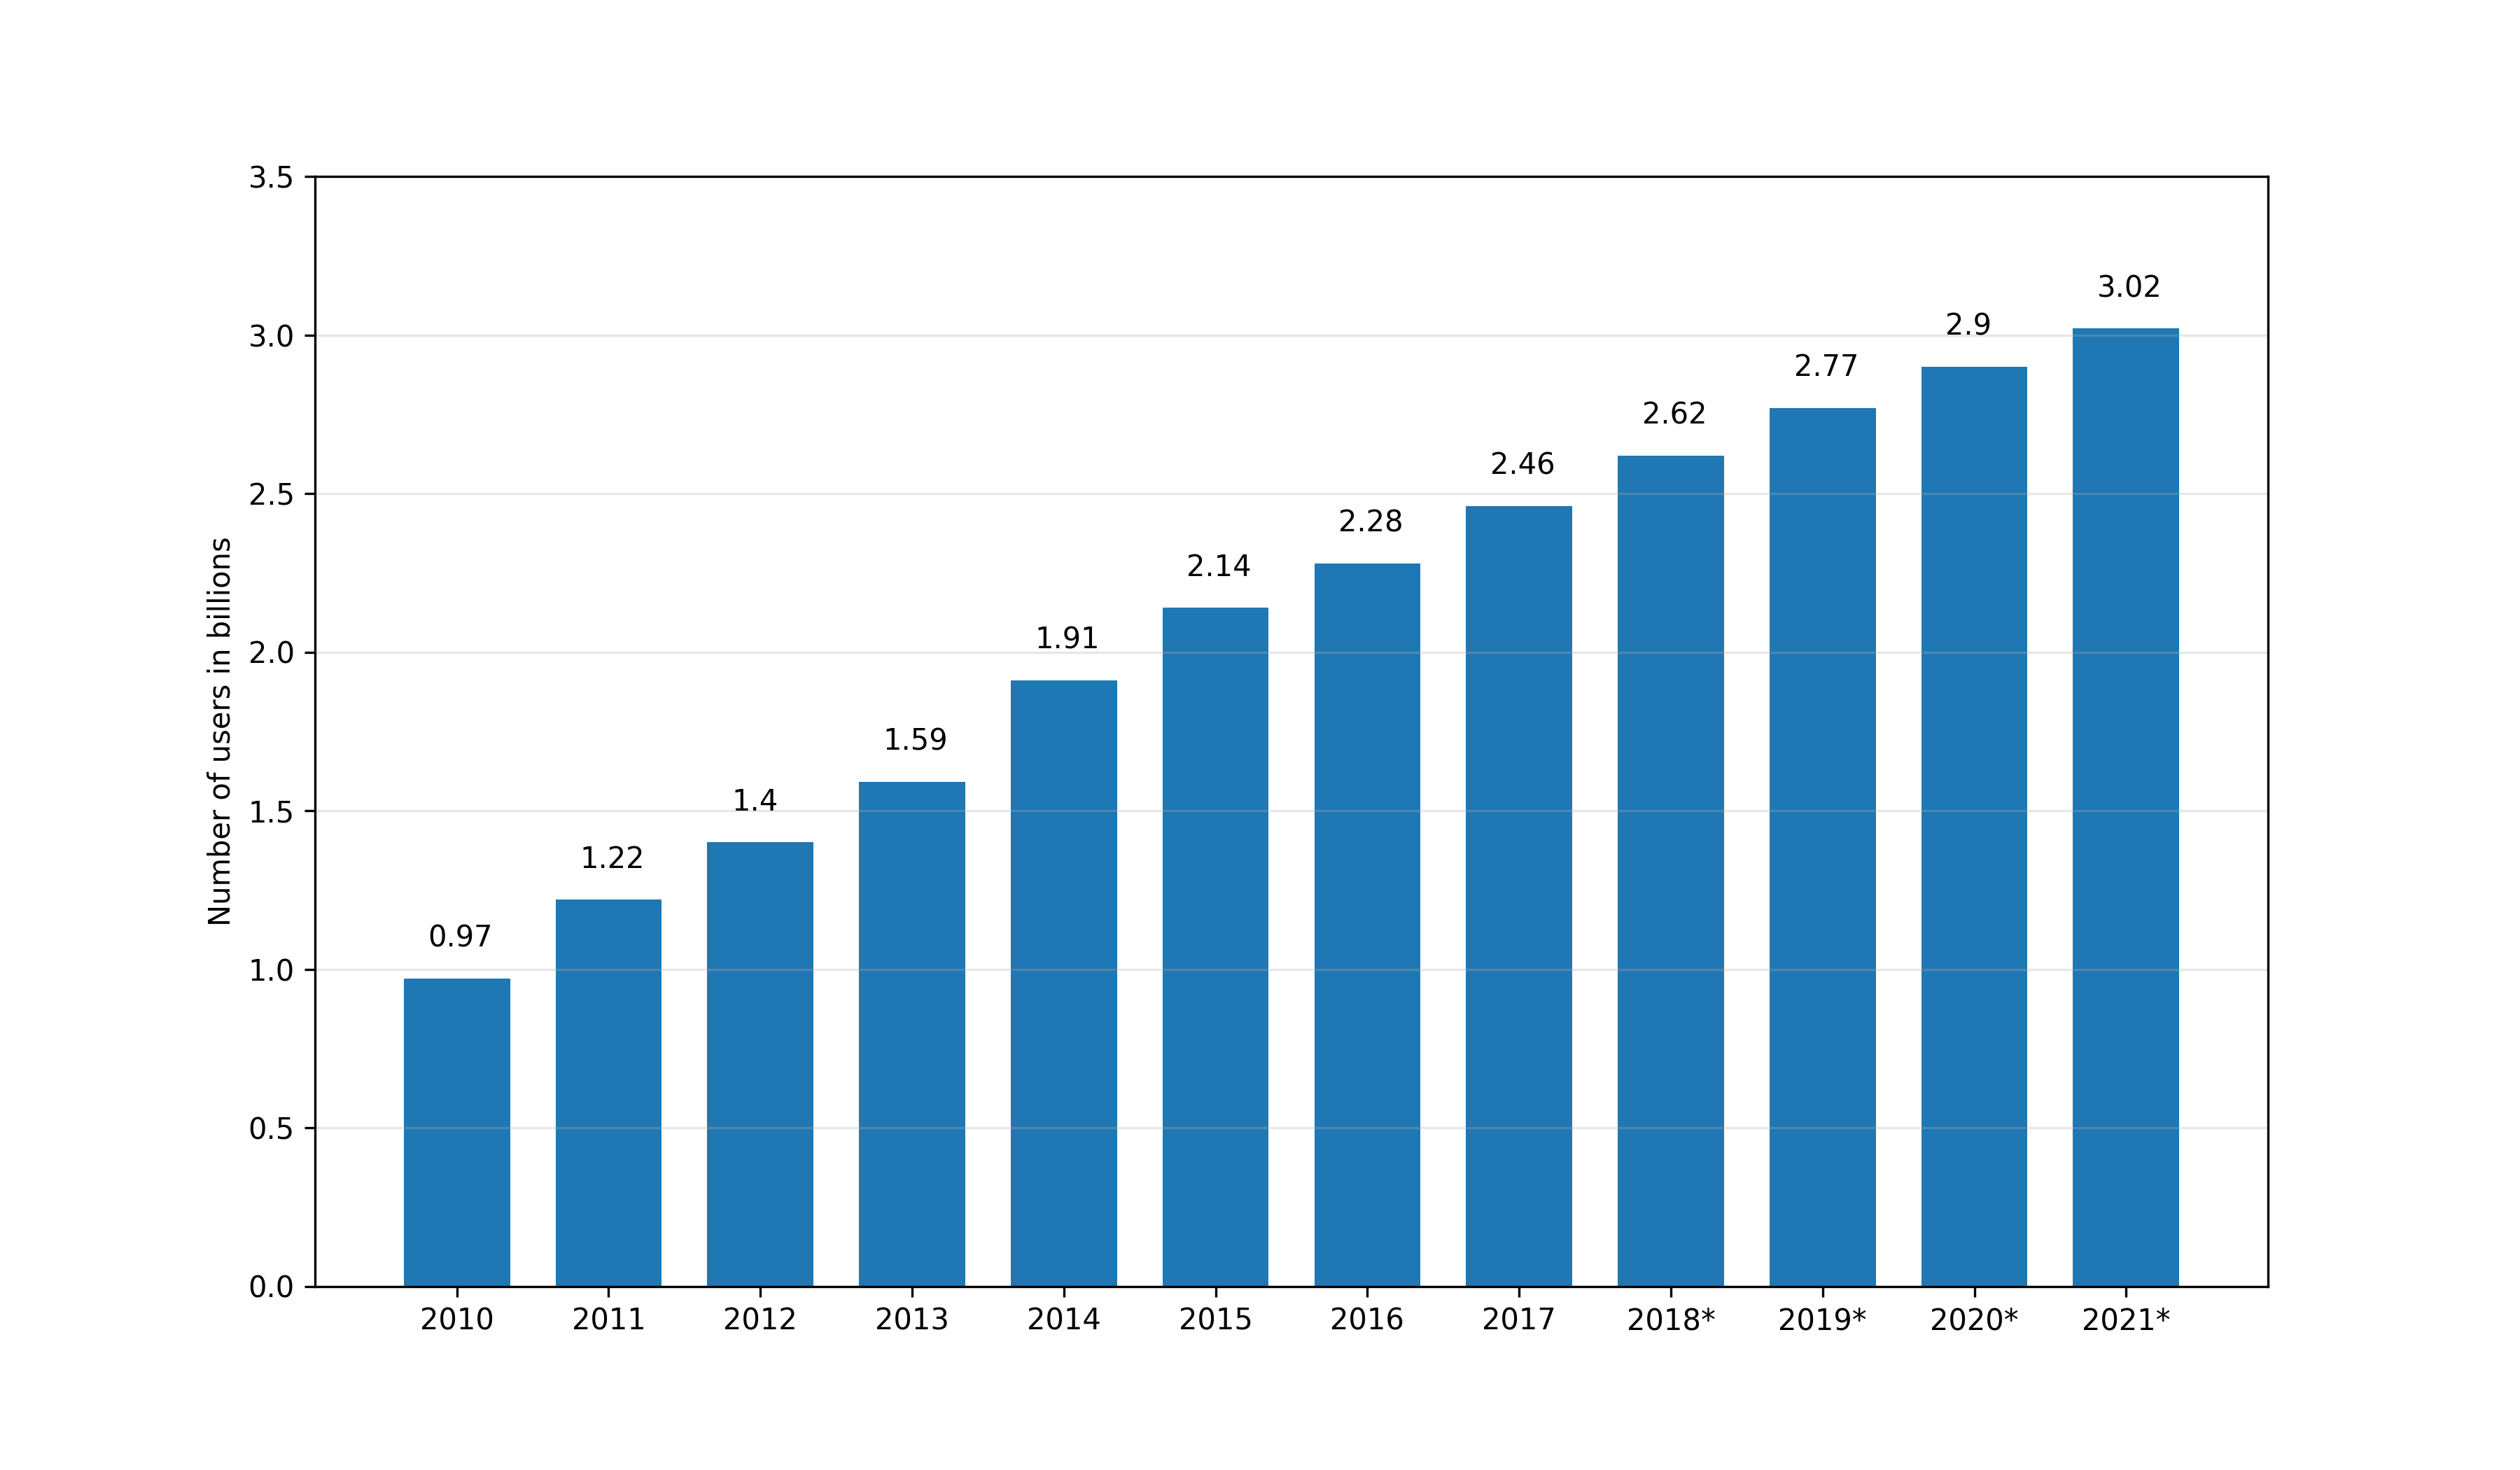
\includegraphics[width=5.5in]{figures/social_media_stat}
	\caption{2010-2021年全球社交媒体用户总数量(以10亿为单位)| 图自:Stataista。}
\end{figure}

在以Facebook\footnote{www.facebook.com}、Twitter、微信\footnote{weixin.qq.com}、微博\footnote{www.weibo.com}为代表的大型在线网络中,网络中的节点数以亿计,网络结构非常复杂,对于巨大规模的高维数据的分析和处理都离不开巨大的储存的计算消耗,从中进行挖掘任务直观上复杂度非常高,而且面对高维数据有可能会产生维数灾难\cite{bellman2015adaptive}(curse of dimensionality)。所谓维数灾难,就是在没有简化参数搜索空间的情况下,对于多参数的函数进行最优化学习时,如果需要得到稳定的参数学习效果,学习样本需要跟随着参数量的增加而指数级的增长,这对于参数学习来说无疑显著地增加了成本。这些问题的原理是因为随着参数量的增加,假设空间不断扩大使得真正有用的数据在空间中的表示非常稀疏。事实上,往往在对事情进行描述刻画的时候,有一种直观的体验,那就是关键特征的选择性描述就会达到足够好的表达效果,而不需要将事物的方方面面描述出来,这样也从另一方面减少信息被淹没的可能,也就是从稀疏的表征空间中得到了真正有用的数据,这种直观的体验引出了数据降维技术。通过数据降维技术可以将特征维度降到合适的量级,可以明显地提高数据分析时候的存储和计算消耗,对于大规模高维数据分析是必不可少的技术手段。

类比在对于网络的描述,当节点数不断增加,用来表示网络的邻接矩阵维度也非常高,基于数据降维的想法,可以不用邻接矩阵的形式将每个节点的所有邻居都描述出来,转而抽象出特定的节点表征形式来包含足够的网络信息。因此,在网络挖掘研究任务中,一个基础的研究工作就是学习有效的节点表征,将网络映射到一个低维向量空间中\cite{chang2015heterogeneous},也就是学习每个节点的低维向量表示,这个过程一般称为图表征(Network Embedding/Representation)。图表征算法属于表征学习,目标就是自动学习从原始特征表示到新的特征表示的一种变换,使得新的特征适合后续的机器学习任务。利用节点的向量表示可以结合机器学习方法进行进一步的挖掘,例如信息检索\cite{weiss2009spectral},节点分类\cite{krizhevsky2012imagenet},聚类\cite{ng2002spectral}等。分类算法作为数据挖掘常用的算法,应用在网络研究之中可以用来对网络中的节点进行分类研究。在网络中的节点分类,分为两个不同的研究问题,即单标签分类问题和多标签分类问题。如果样本实例只能属于某一种类别标签,这种分类问题属于单标签分类问题;如果样本实例可能会属于多种类别标签,这种则属于单标签分类问题。这两种问题在网络研究场景下分别对应不同的情况,比如社交网络中每个用户的标签即为用户所属社区,非重叠社区场景对应单标签分类问题,重叠社区场景则对应多标签分类问题。

在具体的应用场景中,网络中的节点除了各自的邻居集合有所差异以外,节点本身也会有着丰富的属性差异,也即网络的信息除了邻接矩阵以外,还有节点的属性信息。例如:在社交网络中,不同的节点会有不一样的用户名、用户ID、性别、年龄等丰富的属性信息,这些属性信息一定程度上表示用户的属性和性质,这些现实的属性信息在一定程度上回影响局部甚至整体网络的静态属性和动态演化,这些网络一般称之为属性网络。比如,社会网络中互为好友的用户如果有共同的兴趣爱好,那么会更大程度地增强联系。通过对属性信息的处理和分析,可以提取有利于网络挖掘的特征,把网络的拓扑结构信息和节点的属性信息结合起来,可以对后续的学习任务提供更有价值的特征。

除此以外,大部分网络挖掘研究关注的是静态网络。静态网络中节点和边的状态基本不变,而且大部分对于静态网络的研究需要得到完整的网络拓扑结构。与之不同的是,在真实世界中的网络是时刻变化的,新的节点和关系会持续不断加入到网络中,这种网络一般称为流式网络\cite{aggarwal2014evolutionary}。在流式网络中,部分节点的关系是暂时性,比如在邮件或者通信网络中,用户的交互可以用代表节点关系的流数据来表征。持续的流数据需要采用实时的方式来进行分析,全局或者静态的分析手段不再适用。在机器学习领域,对流数据以增量方式进行学习方法称为在线学习或增量学习,就是对新产生的数据样本通过离线训练好的模型进行预测的,同时对离线模型本身也进行更新,从而减少对历史数据重新计算而造成的资源浪费。在对流式网络挖掘和网络演化的研究中,由于网络规模巨大无法将对整个网络进行全局分析,并且要考虑到足够低的时间复杂度,因此对于流式网络的研究非常具有挑战性\cite{zhao2011gsketch,le2012linked}。

%%%%%%%%%%%%%%%%%%%%%%%%%%%%%%%%%%%%%%%
%----------------------------------------     研究现状     ---------------------------------------%
%%%%%%%%%%%%%%%%%%%%%%%%%%%%%%%%%%%%%%%
\section{研究现状}
下面从以下几个方面开始介绍国内外相关研究现状:
\begin{itemize}
\item {图表征学习的意义及相关研究}
\item {属性网络的重要性及相关研究}
\item {增量学习的相关研究}
\item {增量图表征的相关研究}

\end{itemize}

关于图表征算法的研究,最早源自谱聚类(Spectral Clustering )的研究,顾名思义,谱聚类首先是一种聚类方法,具体思想则是通过挑选对应矩阵中的特征值和特征向量来得到节点的表征,谱聚类被广泛地使用在社区发现(Community Detection)\cite{leskovec2010empirical}和图像分割(Image Segmentation)\cite{shi2000normalized}领域。后2000年有人提出流形学习的方式来实现图表征,主要方式是保证网络结构的局部特性来构建近似网络,将问题转化为特征分解的问题,从而实现映射到低维向量空间的目标;在流形学习中最具代表性的几个算法:局部线性嵌入LLE\cite{roweis2000nonlinear}(Locally Linear Embedding)、等距映射ISOMAP\cite{tenenbaum2000global} (Isometric Feature Mapping)和拉普拉斯特征映射LE\cite{belkin2002laplacian}(Laplacian Eigenmaps)。图表征中的LLE算法,假设在网络的局部领域上任意节点的表征向量应该是欧式的,也就是说表征向量是局部线性的。根据这个假设,任意节点的表征向量都可以用它的邻居以加权的形式线性表示出来,在非平凡解的约束下,可以得到LLE的解,可以看出LLE是一种局部流形学习方法。与此不同的是,等距映射ISOMAP的假设是节点表征向量应该使变换前后距离保持不变,而且等距映射ISOMAP是一种全局流形学习方法。而拉普拉斯特征映射跟类似于LLE算法,基本假设是,网络中连边权重较大的节点之间,表征向量越接近,采用二范数对表征向量的接近程度进行衡量,将优化问题变成求解特定矩阵的特征值和特征向量的问题。

在此之后,对于图表征的算法研究开始成为一个新的领域。其中,Google\footnote{www.google.com}在公开发布其词表征算法Word2Vec\cite{mikolov2013efficient}后,DeepWalk\cite{perozzi2014deepwalk}引进自然语言处理中的词向量表征算法,通过网络中的随机游走进行网络采样形成类似语料库的路径集,进而实现对网络节点向量表征的学习。2015年,Tang\cite{tang2015line}提出了一种可扩展的图表征算法LINE,其中提出了一阶接近度和二阶接近度(first-order proximity and second-order proximity)来描述网络结构,一阶接近度相当于描述网络中互为邻居的相似程度,论文中以KL散度(Kullback-Leibler divergence)作为距离函数进行描述,二阶接近度则是用来描述网络中存在共同邻居的节点之间的相似程度,同样以KL散度为距离函数,并基于接近度的组合构建图表征算法需要优化的目标函数,进一步通过优化目标函数实现目标。2016年,Grovel\cite{grover2016node2vec}基于DeepWalk的方式改进了随机游走方式,提出node2vec算法,论文中将随机游走过程更改为具有两个自由度的模型,通过这两个参数分别控制广度优先和深度优先,从而保留网络结构的同质性特征或者结构等价性特征。另外,一些基于矩阵分解的算法\cite{ahmed2013distributed,singh2008relational,zhu2007combining}被提出,其中Shenghuo Zhu等基于PCA,NMF方式提出一种改进的矩阵分解方式,同时在目标函数中结合边信息和属性信息。除此之外,Jiezhong Qiu等\cite{qiu2017network}提出以上方法的统一解释,推导出包括DeepWalk,LINE,PTE\cite{tang2015pte},node2vec在内的四种算法的矩阵分解形式。

单纯基于网络结构本身的研究在应用上存在局限性,因为网络中节点会包含丰富的属性信息,如文本,图片等相关信息,除去从文本,图片中提取特征的基本手段外,如何使这些属性信息更有利于网络表征学习过程也具有非常可观的价值。关于属性网络中图表征算法的研究,在Cheng Yang\cite{yang2015network}和Huang\cite{huang2017accelerated}的研究中,提出合并的特征表示方式,将节点的属性特征和网络结构本身的特征结合起来,从而得到更利于节点分类的向量表征形式,Cheng Yang等在TADW(text-associated Deep Walk)中首次提出并证明DeepWalk的矩阵分解形式,结合文本特征构造目标函数,实现将文本特征融入到网络表征中。在2016年,Zhang\cite{zhang2016collective}提出了一种基于判别矩阵分解的方法,在矩阵分解的目标函数中加入分类的经验损失函数,将分类任务和图表征过程结合起来统一优化,使得到的结果在表征足够多信息的同时,具有良好的分类性能。

在互联网技术发展迅猛的当下,业界以几何倍数地积累着越来越多的数据,数据分析和处理就遇到了一些问题。首先,想要获得大量的标注数据是非常耗费资源的,那么人工标注数据这种手段显然是不可行的,采用机器学习算法自动进行预测分析才是首选。而对于机器学习算法而言,数据增长到一定的规模,模型训练的时间会非常长,这会非常影响用户体验,特别是对于线上的程序,以传统方式对模型重新训练几乎是不可能的。另外最重要一点,对于分类模型,如果出现了一个新的类,那么传统的机器学习算法是无法自动识别的。在意识到传统机器学习的这些问题后,Coppock和Freund在1962年提出了增量学习的概念\cite{coppock1962all},或称为在线学习,这两个概念略有区别,但在本文讨论范围内不作区分。区别于传统算法,增量学习应该具有一些特性:首先,分类器根据新的数据会学习新的信息,也就是说模型会根据新数据进行更新;其次,在增量学习时,用于学习的应该只有新的数据,而不是需要整合原始数据和新数据。 根据文献的不同增量学习算法特征,可以将分类问题的增量学习分为三个种类:样本增量学习(Sample Incremental SIL),类别增量学习(Class Incremental Learning)和特征增量学习(Feature Incremental Learning)\cite{zhong2017survey};其中样本增量学习就是假设不断有新的样本加入,同时数据的特征维度,和预测分类数仍保持不变;类别增量学习顾名思义就是假设预测的类别数有可能变化,在新的数据可能会有新类别产生的;特征增量学习就是假设在数据的特征维度在变化。

大部分的增量学习算法是基于随机梯度下降(Stochastic Gradient Descent)的改进\cite{hazan2007logarithmic, xiao2010dual, mcmahan2011follow},基于在线梯度下降的算法优点在于精度高,但是局限在于即使加上L1正则(L1-Norm)很难产生真正意义上的稀疏解,同时在一些不可微点的迭代会出现问题。于是基于这些局限,提出了一些能改善稀疏性的方案,最简单的方式是梯度截断(Truncated Gradient),设定一个梯度阈值或者参数阈值,当参数小于阈值时直接设为0\cite{langford2009sparse};John Duchi和 Yoran Singer\cite{duchi2009efficient}提出了前向后向切分算法FOBOS(Forward Backward Splitting),算法类似于投影梯度下降,但将迭代过程修改成了两步,第一步更新为经验损失函数的梯度下降过程,第二步更新变成求解一个最优化问题,其中第二个最优化问题首先通过L2-norm限制损失迭代结果的范围,其次再增加正则项对模型复杂度进行限制从而达到稀疏结果,从理论上可以证明,第二步的最优化可以使得模型结果具有稀疏性,FOBOS算法使得在线模型具有了可观的稀疏性和不错的精度,FOBOS算法在特定情况下等同于简单的梯度截断方法。Lin Xiao\cite{xiao2010dual}提出了正则对偶平均算法RDA(Regularized Dual Averaging Algorithm),这个算法本身不同于梯度下降方式的学习算法,改成以一个最优化问题进行权重的更新,相当于在某个特征维度的参数累计梯度平均值低于阈值λ后进行截断,通过调节λ可以在稀疏性和精度之间做权衡。从此可以看到基于梯度下降的FOBOS具有较好精度,但是稀疏性不如RDA算法,于是H. Brendan McMahan提出了FTRL(Follow-the-Regularized-Leader)算法\cite{mcmahan2011follow},FTRL算法在L1正则情况下精度和稀疏性都好于前者,从参数更新的形式上看,FTRL优化的最优化问题跟RDA算法只在额外项上存在差异,通过额外项限定新的参数迭代结果不要离上一步的结果太远。另外一个体系是基于SVM(Support Vector Machine)的增量学习方式,Syed等\cite{syed1999incremental}最新提出的增量式方法基于SVM算法的特性,影响分割超平面的是全部的支持向量,而支持向量的个数相对总体样本而言是非常少的,于是Syed等提出在增量学习过程中,对增量的样本和支持向量一起进行重新训练得到新的分类器,循环迭代得到最后的分割超平面,利用支持向量机的特性而设计的这种增量方法提供在处理海量数据是可以为提供不错的优化的,但是模型也存在着明显的局限,那就是数据集特征本身的分布影响着训练过程甚至训练结果的好坏。为了解决数据集特征分布上的差异引起的模型性能,Ruping\cite{ruping2001incremental}在对原始数据子集和新增数据子集采取不一样的方式,通过在目标函数中对不同子集的间隔设置不同的权重,使得数据特征保持良好稳定的分布,通过实验表明,通过调整得到的分割超平面类似于批处理得到的结果。根据判别误分类的差异,这些算法可以进一步分成软间隔和硬间隔两种。相比之下,软间隔分类器的一个优点是可以减少一部分噪音数据的影响\cite{kivinen2002large}。

同样的情况在网络分析里面也存在。大部分的网络表征学习研究对象都是静态的网络,实际的网络是处在不断变化和演进中的,Li\cite{li2017attributed}基于动态网络的变化是缓慢且持续的假设,提出了一种动态网络中的网络表征算法,在论文中,采用拉普拉斯特征映射(Laplacian eigenmaps)的目标函数,并结合节点属性向量,计算各节点间的属性相似度,构造类似邻接矩阵的属性相似度矩阵,将属性相似度矩阵与邻居矩阵分别进行特征映射,再通过优化映射将两组特征融合起来;在增量场景下利用矩阵摄动理论推导网络表征中特征值和特征向量的增量,从而可以快速得到新的网络表征。增量网络表征过程一定程度上类似于增量的机器学习过程,用来表征网络的邻接矩阵或拉普拉斯矩阵在样本和特征维度上都有增量,因此也存在一些差异。Ling\cite{jian2018toward}基于拉普拉斯特征映射方法提出了一种增量节点分类框架,通过增量的图表征方式获得新增节点的表征向量,同时在分类器上也采用增量的分类模型进行学习任务,实现对于新增节点的快速分类学习。

综上所述,对于现实的网络型数据,利用增量式的表征方式来提取网络结构和节点属性信息,对于学习任务和商业应用是具有明显优势的,本文将针对这个课题进行相关的研究。




%%%%%%%%%%%%%%%%%%%%%%%%%%%%%%%%%%%%%%%
%---------------------------------     本文工作与创新点     ---------------------------------%
%%%%%%%%%%%%%%%%%%%%%%%%%%%%%%%%%%%%%%%
\section{本文工作与创新点}
本文主要研究的问题是在动态变化的增量网络中,通过增量的表征方式对网络结构信息和节点属性信息进行提取,来进行快速的网络挖掘学习。为此本文将围绕这一个话题展开研究和分析,提出可行的方案框架。本节将对本文的全部工作内容作简明的概括,详细的分析和研究将于后文具体展开:


\begin{enumerate}
	\item 针对目前的图表征算法存在的一些问题,本文基于拉普拉斯特征映射提出了一种保留高阶接近度的图表征算法HLE(High-order Laplacian Eigenmaps),通过对节点进行不同方法的相似度计算得到表示高阶接近度的矩阵,来改进低阶接近度在节点分类和链路预测准确率不高的缺点。
	\item 将基于高阶接近度的拉普拉斯特征映射应用于动态更新的网络之中,提出增量学习算法iHLE,通过对网络增量成分的分析对原表征结果进行调整,在保证后续学习任务准确率的同时降低了算法的时间复杂度。
	\item 针对属性网络的节点属性降维算法存在的一些问题,本文提出了一种基于相似度计算的节点属性降维算法SR(Similarity Reduction),并在此基础上提出在增量场景下降维算法(iSR),在真实数据和人工数据集上实验,表现出良好的准确率和时间复杂度。
	\item 结合提出的增量图表征算法和增量节点属性降维算法应用于属性网络,在真实网络中进行节点分类与链路预测,并与业界已有算法进行对比,在保证准确率的同时,能显著降低算法运行的时间成本。
\end{enumerate}






%%%%%%%%%%%%%%%%%%%%%%%%%%%%%%%%%%%%%%%
%-------------------------------------     本文章节安排     ------------------------------------%
%%%%%%%%%%%%%%%%%%%%%%%%%%%%%%%%%%%%%%%
\section{本文组织结构}

本文共分为六章节,具体内容结构如下:

第一章是本文的绪论部分,描述了本文的研究背景和意义、问题相关的研究,以及本文的主要工作内容和创新点。

第二章是相关工作综述,主要介绍的论文主要工作所涉及的一些技术和算法的具体介绍,主要包括图表征算法,属性图表征算法和增量学习算法的一些具体介绍。

第三章提出网络中的增量图表征算法。介绍了基于高阶接近度的拉普拉斯特征映射算法HLE,以及在增量场景下的增量学习算法iHLE,通过对节点进行不同方法的相似度计算得到表示高阶接近度的矩阵,来改进低阶接近度在节点分类和链路预测准确率不高的缺点;同时在增量场景下对表征结果进行调整,在保证后续学习任务准确性的同时降低了算法的时间复杂度。

第四章提出属性网络中的增量图表征算法。介绍基于相似度计算的节点属性降维算法SR,以及在此基础上提出的增量场景下的降维算iSR,在保证后续学习任务准确性的同时降低了算法的时间复杂度。

第五章是实验分析部分,通过实验结合增量图表征算法和增量属性降维方法,在真实网络与人工网络上进行节点分类与链路预测,并跟业界已有算法进行在时间效率和准确率上进行对比分析。

第六章是总结与展望,主要总结了本文的主要工作内容,同时对文中算法的一些不足和改进工作进行分析和展望。

\chapter{相关工作}
本章将对本文的研究框架中所涉及的相关技术进行分析,主要分为三个方面:一个方面是介绍结构图表征的相关算法,也就是单纯对网络的结构进行表征学习的相关技术及其发展演化,第二是对属性网络中相关的图表征算法进行介绍和分析,第三是对增量学习相关的技术细节进行分析。



%%%%%%%%%%%%%%%%%%%%%%%%%%%%%%%%%%%%%%%
%------------------------------------     图表征算法     -------------------------------------%
%%%%%%%%%%%%%%%%%%%%%%%%%%%%%%%%%%%%%%%
\section{结构图表征算法}
图表征(Network Embedding/Representation)过程是通过一定算法获得网络中所有节点向量表征的一个过程,这类算法本身类似于一个完整任务的中间流程,因为没有对应的量化指标去直接衡量图表征算法是否性能突出,图表征算法从某些程度类似于高维数据的降维过程,降维之后需要放入特定的机器学习任务,如节点分类、节点聚类(社区发现)、节点相似度计算、链路预测等,通过学习任务的指标来衡量图表征过程的优良。虽然没有一个公认的量化指标来对图表征算法性能进行评价\cite{goyal2017graph},但是在设计图表征算法的时候需要考虑一些准则来达到利于数据可视化或者后续学习任务的目的,一般而言需要考虑以下几点:
\begin{itemize}
	\item { 对网络性质的保留:有效合理的图表征向量需要能够保留下网络本身的结构特征,比如节点间因为连接而产生的相似度,在向量化表征之后可以得到近似的结果。在这一方面存在的难题是,网络本身的性质存在很多,比如相似度、距离,这些性质在表征向量中不一定能完全兼顾,因此对于不同的图表征算法,其性能好坏取决于后续的具体应用。}
	\item {伸缩性:现实应用中的网络规模非常巨大,大型网络中节点至少都是千万级别的,节点间的连边的量级更是十亿级别的,所以图表征算法的可扩展性是非常具有现实意义的,但是当需要设计一个能保留网络全局信息的图表征算法的时候,设计一个伸缩性性好的算法是非常具有挑战性的。}
	\item {表征向量的维数:对于表征向量来说,挑选一个合适的向量维度是比较困难的。高维向量会保留更多的网络原本的信息,从直观上理解,就相当于减小了舍入误差,但是过高维的向量表征对于学习任务来说其复杂度是不友好的;低维向量表征虽然能优化计算复杂度,但是过低维的向量表征会丢失一部分精度。对于向量表征的维度也是根据学习任务的不同特点来调整的。}
	\item {自适应性:对于大型网络来说,做一次向量表征的计算成本是比较高的,在大型网络中不可忽略的是网络一直在变化演进中,包括网络的结构信息,如新增节点和连边的增删等,还有节点的属性信息都是时刻在变动的,从计算资源和学习任务时效性来讲,新的网络信息不应该重复地进行同样的学习过程,好的网络表征算法应该考虑到网络的动态变化。}
\end{itemize}

\textbf{图表征算法的定义}:给定一个图$G = (V,E)$,$V$表示网络$G$中节点的集合,$E$表示网络$G$中连边的集合,通常图是用邻接矩阵$A \in R^{|V|\times|V|}$表示的,图表征算法的定义就是通过寻找一个映射函数来表征网络中的每个节点:
\begin{equation}
f_G: A \rightarrow R^{|V| \times d} \qquad s.t.\quad d<<|V|
\end{equation}

\begin{figure}
	\centering
	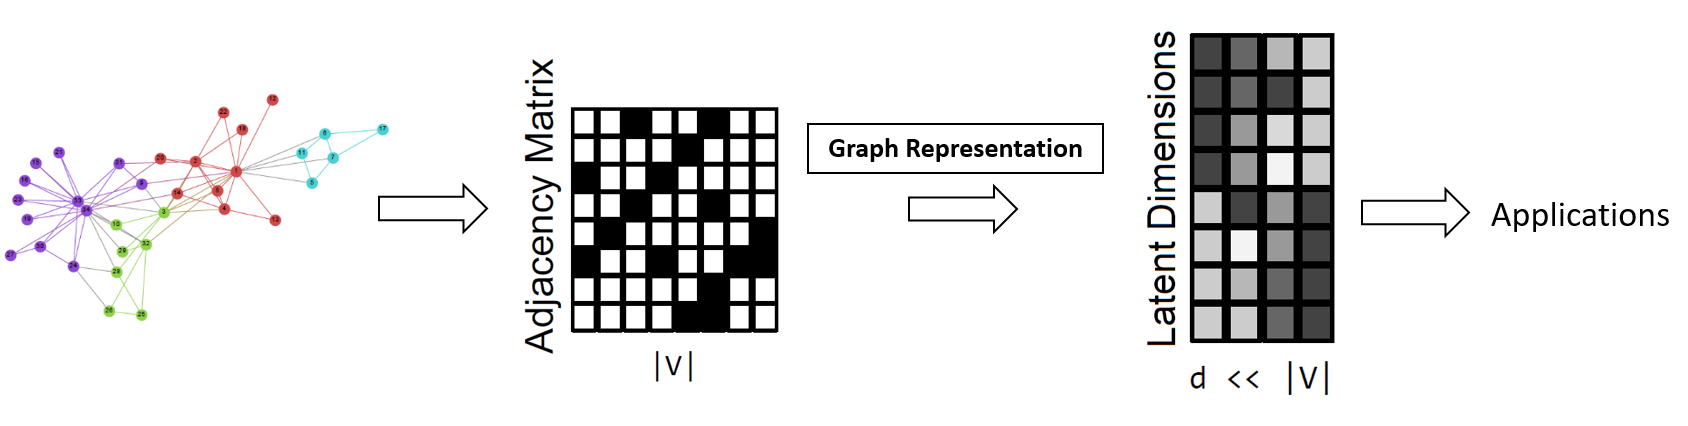
\includegraphics[width=5.5in]{figures/network_embedding}
	\caption{图表征算法}
\end{figure}


网络的邻接矩阵随着图中节点规模的增大,会变得非常稀疏,也就显现出了低秩的性质。对于低秩矩阵的流形学习的思想类似于图表征的过程。流形学习(Manifold Learning)领域提出借鉴拓扑流形的降维方式,这些方法通过设计一些表示节点间关系的矩阵,通过特征值分解的方法来获得表征向量,比如最基础的用来表示节点之间关系的邻接矩阵$A$,拉普拉斯矩阵 $L$(Laplacian Matrix)。通过分析,适用特征值分解的方式,需要矩阵满足对称正定,对于设计不符合要求的矩阵则需要根据随机梯度下降(Stochastic Gradient Descent)去求解。
在2013年,Google的开源工具Word2Vec\cite{mikolov2013efficient}发布之后,借鉴词向量表征的思路,Node2Vec和DeepWalk算法以蒙特卡罗随机游走的方式进行网络路径采样,将采样得到的路径视为词向量表征中的语料库,然后采用类似Word2Vec方法进行学习。在2015年,Jian Tang\cite{tang2015line}在提出LINE算法的同时提出了接近度的概念,根据接近度的概念,可以将不同的图表征算法进行分类。下面主要介绍一下接近度的概念,然后基于接近度的阶数,按从低阶到高阶接近度依次介绍:%局部线性嵌入LLE(Locally Linear Embedding),%
拉普拉斯映射LE(Laplacian Eignemaps) , LINE(Large-scale Information Network Embedding)算法, DeepWalk算法,Node2Vec算法。
\subsection{接近度}
\definition{\textbf{一阶接近度}:}
网络中的一阶接近度是用来描述节点对的局部接近特性。在网络$G$中,对于有连边的节点对($u$,$v$)
连边的权重$W_{uv}$则为一阶接近度(first-order proximity),对于没有连边的节点对,则一阶接近度则为0。

所谓一阶接近度,通常是用来描述网络中节点之间的相似度,直观的理解可以视为一阶接近度用来描述网络的一度邻居结构,也即局部结构,这也是符合常识和具体的应用场景的,例如在社交网络中,有直接联系的节点往往具有更强的亲密度。在获取和交换信息上,用户节点更加倾向于直接作用给一度邻居。基于这一点构想,很多算法基于保留一阶接近度的方法来构造目标函数,然后通过优化目标函数得到所求的表征向量,其中包含IsoMap算法,局部线性嵌入算法,拉普拉斯映射算法,图分解GF\cite{ahmed2013distributed}(Graph Factorization)。

但在现实的网络场景中,一阶接近度是存在局限性的。局限性来源于两方面:第一方面来自于数据收集的问题,收集到的网络数据未必能完全体现物理世界中真实的全部连接数据\cite{liben2007link} ,一些存在直接链接的节点可能在数据收集过程丢失,这种缺失情况在只保留一阶接近度的情况下是存在局限的。第二方面,网络本身的特性使得网络存在路径,节点对之间的路径往往不唯一,用来表示非直接连接节点对之间的相似度一般用最短距离来描述,这种情况对于只保留一阶接近度的图表征来说是很难解决的,从而会损失掉一部分网络的信息;因此在图表征算法中只采用保留一阶接近度的方式对于很好地保留网络的信息是不够的。
\definition{二阶接近度}





%%%%%%%%%%%%%%%%%%%%%%%%%%%%%%%%%%%%%%%
%---------------------------------------     本章小结     ----------------------------------------%
%%%%%%%%%%%%%%%%%%%%%%%%%%%%%%%%%%%%%%%
\section{本章小结}
本章对本文相关的研究工作进行调研,分别从函数与程序库推荐、相似移动应用检测两个方面对现有的相关文献和工作进行分析和讨论。由于本文研究的问题——为开发者推荐合适的第三方库——鲜有相应工作,因此本章对与本文相近的工作进行调研分析。

函数和程序库推荐与本文研究问题相近,其主要目的是在项目工程开发过程,为开发者推荐合适、正确的函数、参数等,以避免错误使用和程序漏洞。相关的程序库推荐主要面向的是传统项目工程(如Java、C\#等),且通过分析项目中已使用的程序库情况,为开发者推荐其他相关的程序库。而本文研究的对象是移动应用,且关注分别在需求分析和后期维护两个阶段对开发者需求进行分析,从而为开发者推荐最合适最优的第三方库。本文研究的场景更广,且主要面向移动应用开发者。

相似移动应用检测是本文研究算法中的重要组成部分,因此本章调研了相关工作,并与本文提出的相似性计算方法进行比较和讨论。在相似移动应用检测工作中,主要分为两类方法,分别是动态检测和静态检测。由于动态检测方法需要在运行环境下对移动应用进行检测,因此需要消耗大量的计算资源,难以在大规模的移动应用数据库上进行扩展和应用。静态检测方法通常从移动应用元数据和程序代码两个角度进行分析检测。移动应用元数据包含多种数据类型,能够表征移动应用的功能特征,特别是描述文本,其通常阐述了与移动应用功能相关的文字信息。但此类方法忽略了移动应用代码层信息,特征涵盖不全,因此在相似性计算中可能有偏差。程度代码则从底层、更细粒度的角度体现了移动应用的功能信息,通过分析程序中各函数间的依赖关系,能够提取移动应用在代码层面的特征。但在程序依赖图构建过程中,需要消耗大量计算资源,无法实现快速高效识别。

现有的方法,多仅从元数据或程序代码角度对移动应用进行相似性分析,鲜有同时从本文和视图两个角度对移动应用进行特征提取,因此本文将在第四章中给出本文提出的基于文本和视图的移动应用相似性计算,从而为开发者推荐合适优质的第三方库。




	
%%%%%%%%%%%%%%%%%%%%%%%%%%%%%%%%%%%%%%%
%----------------------------------------     网络中的增量图表征算法     ---------------------------------------%
%%%%%%%%%%%%%%%%%%%%%%%%%%%%%%%%%%%%%%%
\chapter{网络中的增量图表征算法}
\section{引言}
	社交网络的蓬勃发展使得信息网络研究领域面临越来越多的机遇和挑战。传统的网络特征的表示方法都是以邻接矩阵,拉普拉斯矩阵等离散型或者以中心度,出入度等人工规则来表达,然而在社交网络中随着网络节点的增加,这些表达方法的复杂度和有效性都会出现比较大的问题。近年来机器学习、人工智能的飞速发展,复杂信息网络也因此受益,对网络的表征学习吸引了越来越多的研究兴趣。类似于自然语言中的词向量表征的发展,单词的词频或逆文档频率(TF-IDF)等人工规则表征对于一个单词的描述太过简略,词向量表征则将单词映射成一个向量,向量之间可以计算相似度、并进行加减等操作,对于词的描述在数学意义上更加丰富,图表征学习也是需要从对网络的离散型或人工规则型表达发展出连续性且具有更丰富表征意义的向量表示算法。对于图表征得到的节点表征向量矩阵,需要应用于后续的机器学习任务,不同的机器学习任务对应不同的图挖掘问题,比如对节点向量进行聚类学习,相当于图挖掘领域的社区发现过程;对网络中连边进行分类任务,相当于图挖掘领域的链路预测任务。另外,图表征向量矩阵可用于计算相似度、节点分类、可视化、节点推荐等任务。
	
	本章将提出一种基于高阶接近度的图表征算法,并通过分析不同增量场景的模型变化,提出在增量场景下对应的表征算法。
	
\section{问题描述}
假设一个无向网络$G=(E,V)$,其中$V$表示网络$G$中节点的集合,$E$表示网络$G$中连边的集合,通常图是用邻接矩阵$A \in R^{|V|\times|V|}$表示的,图表征算法的定义就是通过寻找一个映射函数来表征网络中的每个节点:
\begin{equation}
f_G: \textbf{A} \rightarrow \textbf{X} \in R^{|V| \times k} \qquad s.t.\quad k<<|V|
\end{equation}
对于真实应用中的网络往往是存在动态变化的,对于传统的图表征算法来说,真实场景下的动态网络会带来很大的挑战,传统算法基本都是离线模型,当新数据进入时,需要重新对全部数据进行批量处理。在网络规模很大时,离线模型是不具备伸缩性的,也不适合于在线应用中使用。因此对于大型动态网络需要提出一种增量式的学习框架来实现快速、可扩展的表征学习。

为了方便描述统一字符使用规范及意义,用大写字母加粗表示矩阵,如$\textbf{A}$;用小写字母加粗表示向量,如$\textbf{a}$;用普通小写字母代表标量,如$a$;矩阵$\textbf{A}$的第$i$行用$\text{A}(i,:)$表示;矩阵$\textbf{A}$的第$j$列用$\textbf{A}(:,j)$表示,也可以简写为$\textbf{A}_j$;矩阵$\textbf{A}$中第$i$行第$j$列元素用$\textbf{A}(i,j)$表示,也可以简写为$\textbf{A}_{ij}$,矩阵$\textbf{A}$的转置记为$\textbf{A}^T$,矩阵$\textbf{A}$的迹记为$tr(\textbf{A})$,$\textbf{I}$代表单位矩阵;常用的字符表如下表:
\begin{table}
	\centering
	\caption{常用字符及其代表含义}
	\begin{tabular}{|C{1.8in}|C{3.3in}|}
		\hline
		\textbf{字符} & \textbf{含义} \\ \hline\hline
		$G^{(t)}$ & 时刻$t$时的网络数据 \\ \hline
		$G^{(t+1)}$& 时刻$t+1$时的网络数据  \\ \hline
		$\textbf{A}^{(t)}$ & 时刻$t$时网络的邻接矩阵 \\ \hline
		$\textbf{A}^{(t+1)}$ & 时刻$t+1$时网络的邻接矩阵 \\ \hline
		$\Delta\textbf{A}$ & 时刻$t$到时刻$t+1$之间邻接矩阵的变化 \\ \hline
		$\textbf{X}^{(t)}$ & 时刻$t$时网络的表征向量矩阵 \\ \hline
		% $\textbf{X}^{t+1}$ & 时刻$t+1$时网络的表征向量矩阵 \\ \hline
		$k$ & 节点向量表征的维数  \\ \hline
	\end{tabular}
\end{table}

用$V^{(t)} = \{v_1, v_2,\cdots,v_n\}$表示在时刻$t$网络$G^{(t)}$中的节点集合,用$\textbf{A}^{(t)}$来表示时刻$t$的网络结构,随着时刻$t$的变化,网络的拓扑结构会发生变化,当网络中节点数目不变时,用$\Delta\textbf{A}$表示邻接矩阵从时刻$t$到时刻$t+1$的变化;当网络中有新增节点的时候,需要对邻接矩阵$\textbf{A}^{(t)}$进行增广再计算变化量。如前文中提到的,在动态网络中重复用离线模型是不适合在线应用的,那么对于动态网络的学习过程应该分成两个部分:1.静态网网络的学习过程;2.增量网络的学习过程;也即转化成如下两个问题:
\begin{itemize}
	\item \textbf{问题1}:静态场景下的图表征算法。给定网络的邻接矩阵$\textbf{A}^{(t)}$,对于所有节点学习网络的表征向量矩阵$\textbf{X}^{(t)}$。
	\item \textbf{问题2}: 增量场景下的图表征算法。给定网络某时刻$t+1$的邻接矩阵$\textbf{A}^{(t+1)}$,
		和上一时刻的表征向量$\textbf{X}^{(t)}$,对于所有节点学习网络的表征向量矩阵$\textbf{X}^{(t+1)}$
\end{itemize}

下面章节将就这两个问题展开讨论分析。

%%%%%%%%%%%%%%%%%%%%%%%%%%%%%%%%%%%%%%%
%----------------------------------------     静态场景下的图表征算法     ---------------------------------------%
%%%%%%%%%%%%%%%%%%%%%%%%%%%%%%%%%%%%%%%

\section{静态场景下的图表征算法}
在图表征学习中,最早的方法借鉴与流形学习(manifold learning)的算法,其中Belkin和Niyogi提出的拉普拉斯特征映射是流形学习中的一种典型算法,该算法假设表征映射后得到的表征向量需要保证原网络中一阶接近度,也就是需要保证网络中互为邻居的节点对连边权重越大,那么在表征向量空间就应该保证越接近,也即优化如下问题:
\begin{equation}\label{laplacian_st}
\begin{aligned}
\min_{X^TDX=I} \phi(X) &= \frac{1}{2}\sum_{i,j}|X_i - X_j|^2A_{ij} \\
&= \frac{1}{2}(\sum_{i,j}(x_i^2+x_j^2-2x_ix_j) A_{ij}) \\
&=\frac{1}{2} (\sum_ix_i^2D_{ii} +\sum_j x_j^2 D_{jj} - 2\sum_{i,j}x_i x_j A_{ij}) \\
&= tr(X^TLX)
\end{aligned}
\end{equation}
其中$X$为表征向量矩阵,$A$为图的邻接矩阵,$D$为对角元素为节点度的对角阵,$L$为拉普拉斯矩阵。对式(\ref{laplacian_st}),根据谱图理论\cite{chung1997spectral}可以通过拉普拉斯算子的最值特征向量来进行逼近,上述问题可以转化为(推导过程如式(\ref{laplacian_reduce})):
\begin{equation}
\max_{X^TX = I} tr(X^TWX)
\end{equation}
其中$W = D^{-\frac{1}{2}}AD^{-\frac{1}{2}} $。为得到图表征向量就转变成求$W$矩阵的前$k$大的特征值所对应的特征向量。

拉普拉斯特征映射假设中只考虑到保留一阶接近度,对于图表征来说,一阶接近度所表征的信息是远远不够的,因此需要引进更高阶的接近度来表征向量,比如LINE算法引入了二阶接近度;DeepWalk算法引进了$l$(游走半径)阶接近度,对比实验也验证了在保留高阶接近度的算法中后续的节点分类等机器学习任务效果更好。

\subsection{基于高阶接近度的拉普拉斯特征映射}
在这一部分,主要集中在无向图中的图表征过程,因此在保证得到节点的表征向量的同时,对称性也在考虑之列。基于对称性这个基本假设,提出基于拉普拉斯特征映射改进的目标函数,用来保留高阶接近度:
\begin{equation}\label{high_order_condition}
%\begin{aligned}
	\min_{X^TD'X=I} \phi(X) = \frac{1}{2}\sum_{i,j}|X_i - X_j|^2S_{ij} 
%	&= \frac{1}{2}(\sum_{i,j}(y_i^2+y_j^2-2y_iy_j) S_{ij}) \\
%	&=\frac{1}{2} (\sum_iy_i^2D'_{ii} +\sum_j y_j^2 D'_{jj} - 2\sum_{i,j}y_i y_j S_{ij}) \\
%	&= tr(X^T(D'-S)X)
%\end{aligned}
\end{equation}
其中约束条件中的$D'$为区别于$S$矩阵为邻接矩阵时对应的对角矩阵$D$,根据不同的$S$矩阵进调整。$S$矩阵是通过保留高阶接近度的计算方法得到的,比如共同邻居(Common Neighbors,CN)\cite{newman2001clustering}、Adamic-Adar系数(AA)\cite{adamic2003friends}、资源分配系数(Resource Allocation,RA)\cite{zhou2009predicting}、Jaccard系数、Katz系数、个性化Pagerank(Personalized Pagerank)\cite{wang2015link}等方式,后文将称$S$矩阵为\textbf{相似度矩阵$S$}。下面将重点介绍前三种计算方法。

\definition{\textbf{共同邻居}:}
共同邻居计算方法是目前用来衡量节点接近度中使用最广泛的之一,因为这种计算非常简单,节点对$i$,$j$之间的共同邻居值就是跟$i$,$j$都有直接连边的节点数,也即:
\begin{equation}
	CN(i,j) = |N(i) \cap N(j)|
\end{equation}
其中$N(i)$表示节点$i$的邻居节点集合,$|\cdot|$表示对集合计数。将共同邻居这个计算方法推广至矩阵形式,可以得到用来保留高阶接近度的相似度矩阵$S_{CN}$:
\begin{equation}
	S_{CN}(A) = A^2
\end{equation}
其中$A$为无向网络的邻接矩阵。
\definition{\textbf{Adamic-Adar系数}:}Adamic-Adar系数最先是由Adamic和Adar提出来用来计算两个网页之间的相似度的,后来被广泛应用与社交网络分析之中。Adamic-Adar系数的计算方法类似于共同邻居,不同的是对不同的共同邻居采用不同的权重,该系数假定度较高的节点在共同邻居中所占权重较低,权重值为对数节点度的倒数,也即:
\begin{equation}
	AA(i,j) = \sum_{u \in N(i)\cap N(j)} \frac{1}{\log(|N(u)|)}
\end{equation}
其中$|N(u)|$也称为节点$u$的度。同样地,将Adamic-Adar系数计算方法推广至矩阵形式,可以得到对应用来保留高阶接近度的相似度矩阵$S_{AA}$:
\begin{equation}
	S_{AA}(A) = A \cdot M \cdot A
\end{equation}
其中$M$为对角矩阵,且有:
\begin{equation}
M_{ii} = 1/\log(\sum_j{A_{ij}})
\end{equation}

\definition{\textbf{资源分配系数}:}资源分配系数最早是基于物理过程中的资源分配得来的一个计算法方法,过程类似于Adamic-Adar系数的计算方法,同样是给度较高的节点惩罚权重,资源分配系数采取的权重是节点度的倒数,因此可以看出来资源分配系数对度高的节点惩罚相较之下比较重,度处在平均水平的节点两中计算方法的惩罚权重相当。资源分配系数的计算方法如下:
\begin{equation}
	RA(i,j) =  \sum_{u \in N(i)\cap N(j)} \frac{1}{|N(u)|}
\end{equation}
同样地,可以将资源分配系数推广至矩阵形式,得到可以用来保留高阶接近度的相似度矩阵$S_{RA}$:
\begin{equation}
	S_{RA}(A) = A\cdot K \cdot A
\end{equation}
其中$K$为对角矩阵,且有:
\begin{equation}
	K_{ii} = 1/\sum_jA_{ij}
\end{equation} 

根据以上三种系数的介绍和定义\ref{first_order}和定义\ref{second_order}中介绍的接近度概念,在共同邻居的计算方法中引入了二阶接近度,也即二度邻居的信息,在Adamic-Adar系数和资源分配系数中,不仅计算了共同邻居,还对共同邻居的度(邻居总数)进行了计算和处理,也即处理了高于二阶接近度的高阶接近度信息。为方便后文进行推导,可以将三种相似度矩阵$\textbf{S}$计算方法表达成统一的形式:
\begin{equation}\label{unify}
	\textbf{S} = \textbf{A} \cdot \textbf{M} \cdot \textbf{A}
\end{equation}
对应的三种相似度矩阵$S$的表格如下:
\begin{table}
	\centering
	\caption{三种相似度矩阵计算方法}
	\begin{tabular}{|C{1.0in}|C{1.8in}|C{1.8in}|}
		\hline
		$\textbf{S}$ & 表达式 & $\textbf{M}$的值  \\ \hline\hline
		$\textbf{S}_{CN}$ & $\textbf{A}\cdot \textbf{M}_{CN} \cdot\textbf{A}$ & $\textbf{I}$  \\ \hline
		$\textbf{S}_{AA}$ & $\textbf{A}\cdot \textbf{M}_{AA}\cdot \textbf{A}$ & $\textbf{M}_{ii} = 1/\log(\sum_j{\textbf{A}_{ij}})$ \\ \hline
		$\textbf{S}_{RA}$ & $\textbf{A}\cdot \textbf{M}_{RA}\cdot \textbf{A}$ & $\textbf{M}_{ii} = 1/\sum_j\textbf{A}_{ij}$ \\ \hline
	\end{tabular}
\end{table}

考虑式\ref{high_order_condition},当采用不同的相似度矩阵$S$时,$D'$满足:
\begin{equation}
D'_{ii} = \sum_j{S_{ij}}
\end{equation}
于是同式(\ref{laplacian_reduce})推导,则原问题变成:
\begin{equation}\label{decomp}
\max_{X^TX = I} tr(X^TWX)
\end{equation}
其中$W = D^{\prime-\frac{1}{2}}SD^{\prime-\frac{1}{2}}$,上述问题转化为求矩阵$W$的特征值问题,也即对矩阵$W$进行特征值分解:
\begin{equation}\label{evol}
	W = X^T \Lambda X 
\end{equation}
其中$\Lambda$为对角矩阵,对角线元素为矩阵$W$的特征值,$X$为正交矩阵,也即表征向量矩阵。对于式(\ref{decomp})的最大值问题相当于求解$W$最接近特征值分解形式,也即矩阵$X$为$W$前$k$个特征值对应的特征向量组合而成的矩阵。

\subsection{HLE算法描述}
	给定图数据$G = (E,v)$和图表征向量维数$k$,其中图$G$以邻接矩阵$A\in R^{|V|\times |V|}$表示,HLE算法将得到图$G$的向量表征$X\in |V|\times k$。
	
	在算法开始时,根据相似度准则的选择,令相似度矩阵$S$分别为共同邻居$S_{Cn}$、Adamic-Adar系数$S_{AA}$或资源分配系数$S_{RA}$中的一个。根据$S$矩阵计算出对应的对角矩阵$D\prime$,使得$D'_{ii} = \sum_j S_{ij}$。

	进一步计算矩阵$W$,使得$W=D^{\prime-\frac{1}{2}}SD^{\prime-\frac{1}{2}}$,对W矩阵进行特征值分解得到前k个最大特征值对应的特征列向量$\{X_1,X_2,\cdots,X_k\}$,组合成图表征向量矩阵$X$。
	
	HLE算法中根据不同的接近度要求可以选择不同的相似度计算方法,其中共同邻居保留二阶接近度,Adamic-Adar系数和资源分配系数保留网络的三阶接近度。


%\algorithm{基于高阶接近度的拉普拉斯特征映射HLE}
\begin{figure}[htb]
	\centering
	\begin{minipage}{.7\linewidth}
		\begin{algorithm}[H]
			\small
			\caption{HLE算法}
			\begin{algorithmic}[1]
				\Require
				\Statex $\mathcal{A}$ :邻接矩阵
				\Statex $k$ : 表征向量维数
				\Ensure
				\Statex $\mathcal{X}$ :表征向量矩阵
				\Statex
				\State $\mathcal{S} \leftarrow S_{CN}(A) /S_{AA}(A) / S_{RA}(A)$
				\State $D'_{ii} = \sum_j S_{ij}$
				\State $W \leftarrow  D^{\prime-\frac{1}{2}}SD^{\prime-\frac{1}{2}}$
				\State 通过特征值分解得到$W$前k个特征向量,组合成矩阵 $\mathcal{X}$
				\State 返回 $\mathcal{X}$
			\end{algorithmic}
		\end{algorithm}
	\end{minipage}
\end{figure}
%%%%%%%%%%%%%%%%%%%%%%%%%%%%%%%%%%%%%%%
%----------------------------------------     增量场景下的图表征算法     ---------------------------------------%
%%%%%%%%%%%%%%%%%%%%%%%%%%%%%%%%%%%%%%%

\section{增量场景下的图表征算法}
前面一节提出了应用高阶接近度的拉普拉斯特征映射方法来对网络进行表征,对于真实应用中的网络往往是存在动态变化的。比如在社交媒体上,网络中时刻会存在用户进行更新状态、添加好友等操作,这些操作都是会引起社交关系发生变化的,从数学角度看就是网络中的连边会出现增删等情况;除此之外社交媒体中,也会存在有新的用户注册加入的情况,这种情况即对应网络中有新加入的节点。对于传统的图表征算法来说,真实场景下的动态网络会带来很大的挑战,传统算法基本都是离线模型,对于变化后的网络只能进行重新计算或学习,当网络规模很大时,离线模型是不具备伸缩性的,也不适合于在线应用中使用。因此对于大型动态网络需要提出一种增量式的学习方式来实现快速、可扩展的表征学习。

下面将提出一种增量的图表征算法,应用于增量场景下的图表征学习,在这里本文采用文献\cite{chi2007evolutionary}中采用的假设,认为在时刻$t$和时刻$t+1$之间网络的变化是平缓而微小的。如前文中提到的,网络中的变化场景分两类:1. 节点数不变,网络连边的增删;2.节点数的新增;因此下面将分别就这两种情况进行分析和处理。

\subsection{节点数不变}
本文的研究对象是无向网络,根据式(\ref{evol}),在时刻$t$网络表征学习相当对矩阵$\textbf{W}^{(t)}$进行特征值分解,也即:
\begin{equation}
	\textbf{W}^{(t)} = \textbf{X}^{(t)T} \Lambda^{(t)} \textbf{X} ^{(t)}
\end{equation}
其中$\textbf{X} ^{(t)}$为时刻$t$是网络的表征向量,其中$\textbf{W}^{(t)} = \textbf{D}^{\prime(t)-\frac{1}{2}}\textbf{S}^{(t)}\textbf{D}^{\prime(t)-\frac{1}{2}}$;在网络节点不变的情况下,用$\Delta\textbf{W}$表示随机





根据式(\ref{unify})对不同个相似度矩阵的统一表示,



%%%%%%%%%%%%%%%%%%%%%%%%%%%%%%%%%%%%%%%
%----------------------------------------     本章小结     ---------------------------------------%
%%%%%%%%%%%%%%%%%%%%%%%%%%%%%%%%%%%%%%%
\section{本章小结}
本章从统计学角度,通过对实际数据的分析,深入探讨了第三方库与移动应用的关系。评分作为移动应用最重要的评价方式之一,是开发者最为关注和在意的方面。因此,任何能够提高移动应用评分的方式都具有现实意义和价值。第三方库作为本文的研究对象,其与移动应用评分的关系是本文研究的基础和出发点。本章的分析,其目的是为了对本文研究问题的依据进行验证。为了比较不同评分的移动应用间使用第三方库的差异,本章将移动应用根据评分高低分成了四个类别,然后对这四个类别的移动应用,分别从第三方库的个体使用量和平均使用量两个方面进行检验分析。检验结果显示了高评分类别的移动应用与低评分类别的显著差异。本章亦对高评分类别的移动应用进行更为细粒度的分析,从一星作为步长减少到半星作为步长,将高评分类别的移动应用分成更小的四个集合。在此基础上,通过两两对比检验,结果表现出与预想一致的结果,即在高评分类别中,就第三方库使用情况,其内部同样具有显著的差异。经过大小对比组的检验分析,本章得出以下结论:\textbf{使用第三方库的移动应用确实具有更高的评分。}此结论回答了本章开始的研究问题,且验证了本文研究问题的依据,为本文的研究工作奠定了基础。本章的检验分析结果可以为其他研究者所用,为其之后在第三方库相关问题的研究中提供数据支撑。


%%%%%%%%%%%%%%%%%%%%%%%%%%%%%%%%%%%%%%%
%----------------------------------------     算法     ---------------------------------------%
%%%%%%%%%%%%%%%%%%%%%%%%%%%%%%%%%%%%%%%
\chapter{算法}
本文希望通过分析移动应用开发者的需求,为其推荐高质量、功能相关的第三方库,以协助其快速开发优质的移动应用,从而吸引用户并增加收益。本文从移动应用开发流程的两个阶段入手,即需求分析和后期维护,分析获取开发者的需求。具体而言,在需求分析阶段,主要利用移动应用的描述作为输入信息,通过分析描述这一文本数据,从而提出其中所包含的移动应用的功能信息;在后期维护阶段,由于已经有早期开发的移动应用的版本,因此该版本所包含的功能信息可以从其视图界面、程序代码等方面获取。所提取的功能信息均用以表征开发者的需求,从而可以通过聚类的方法,将相似功能的移动应用聚集到一起。所聚集的移动应用具有很强的相似性,相似的移动应用可以为开发者提供参考和借鉴,特别是质量较好、评分较高的移动应用,其所使用的第三方库便是可以为开发者提供参考之处。通过该方法分析获得的第三方库,是开发者所需的且优质的第三方库,因而可以推荐给开发者使用。

本章将对本文研究的问题作具体定义,明确问题的背景及目标,详细内容将在4.1节中阐述。在明确研究问题的目标后,本章将针对研究问题给出本文的解决方法。解决方法包括三分部分:相似性计算、移动应用聚类、第三方库推荐,算法的整体框架将在4.2节中详细阐述。其中,相似性计算将根据移动应用开发流程的不同阶段,对不同的信息源进行分析计算。在需求分析阶段,本文将通过分析移动应用的描述来获取功能需求,因而需对描述文字进行自然语言处理和分析,并依此计算移动应用(功能)的相似性,具体计算方法将在4.3节中阐述。在后期维护阶段,本文将通过分析现有版本的移动应用的视图界面来获取功能信息,因而需对移动应用的程序包文件进行处理,并从程序代码层面对移动应用内部信息进行分析,从而计算移动应用间的相似性,具体实现算法将在4.4节中详细描述。基于计算获得的移动应用的相似性,本文使用聚类算法把功能相似的移动应用聚集到一起,聚类算法和过程将在4.5节中阐述。最后,本文的最终目标——为开发者推荐优质可靠的第三方库——将在4.6节中展开讨论,基于前两部分的相似性计算和移动应用聚类,本文可以准确地定位开发者的需求,并根据相似移动应用使用第三方库的情况,为开发者匹配最佳的第三方库。下文将对以上几个部分内容分别展开讨论。



%%%%%%%%%%%%%%%%%%%%%%%%%%%%%%%%%%%%%%%
%----------------------------------------     问题定义     ---------------------------------------%
%%%%%%%%%%%%%%%%%%%%%%%%%%%%%%%%%%%%%%%
\section{问题定义}
本文主要研究的问题是为移动应用开发者推荐优质、合适的第三方库。因此,需要对移动应用和第三方库,以及相关问题进行定义。首先,给定移动应用集合$\mathcal{A}$,其中任意一个移动应用为$\mathbf{a}_i \in \mathcal{A}$。为了协助开发者寻找最合适的第三方库,则需要对开发者的需求进行分析。本文分别对两个不同阶段的需求进行分析,分析内容包括移动应用描述和视图信息。对于任意一个移动应用$\mathbf{a}_i$,其描述的文本信息表示为$\mathbf{t}_i$,视图信息表示为$\mathbf{v}_i$,则移动应用可表示为由描述和视图组成的特征集合$\mathbf{a}_i = \{\mathbf{t}_i, \mathbf{v}_i\}$。由于描述和视图属于两个不同的开发阶段,因此本文在对移动应用实际操作过程中,分别表示为$\mathbf{a}_i = \{\mathbf{t}_i\}$和$\mathbf{a}_i = \{\mathbf{v}_i\}$。但此两项特征的基本概念和依据相同,故在此不做区分。

对开发者需求的分析,本文是通过搜寻相似移动应用的方式来解决的。具体而言,为给开发者推荐第三方库,本文先对移动应用市场上已有的移动应用进行分析,了解统计不同类别、不同功能的移动应用所使用的第三方库情况。一个移动应用可能使用多个第三方库。例如,一个常用的社交移动应用,其可能使用的第三方库包括聊天界面展示、定位服务、数据库管理等。因此,对任意一个第三方库定义为$l_j \in \mathcal{L}$,其中$\mathcal{L}$为所有移动应用可能使用的第三方库集合。那么,一个移动应用所使用的第三方库可以表示为$\mathbf{l}_i = \{l_{i,1}, l_{i,2}, ..., l_{i,n}\}$。在此基础上,本文将与开发者需求相近的移动应用筛选出来,这些移动应用所使用的第三方库便进入后续推荐的候选名单。因此,在搜寻相似移动应用的过程中,本文定义移动应用相似性如下:
\begin{definition}[移动应用相似性]
给定一个移动应用集合$\mathcal{A}$,移动应用相似性计算的目标函数为$f:\mathcal{A} \times \mathcal{A} \rightarrow \mathbb{R_+}$,其中$f(\mathbf{a}_i, \mathbf{a}_j)$表示移动应用$\mathbf{a}_i$与$\mathbf{a}_j$间的相似性。
\end{definition}

为了筛选相似的移动应用,通常的解决方法是将功能相近的移动应用进行聚类。因此,本文根据移动应用的相似性,对其进行聚类操作,聚类过程将在4.5节详细阐述。聚类后的移动应用将被分成$k$个集合,表示为$\mathcal{S} = \{S_1, S_2, ..., S_k\}$,每个集合中的移动应用互相间都具有相似的功能。因此,相应集合中的移动应用所使用的第三方库同样呈现类似的关系。最终,研究问题转化成如何从一组功能相似的移动应用中找到对开发者有用的第三方库。就该问题,本文根据开发者所需开发的移动应用$\mathbf{a}_t$所在集合$S_i$(聚类后的所在集合),使用协同过滤算法,筛选出最可能被开发者采纳的第三方库,并将此列表推荐给开发者。至此,本文整个研究问题已定义清楚,下面将详细介绍本文对各个问题的具体解决方案和步骤。



%%%%%%%%%%%%%%%%%%%%%%%%%%%%%%%%%%%%%%%
%----------------------------------------     算法框架     ---------------------------------------%
%%%%%%%%%%%%%%%%%%%%%%%%%%%%%%%%%%%%%%%
\section{算法框架}
\begin{figure}
	\centering
	\includegraphics[width=5.7in]{figures/architecture}
	\caption{TV-LibRec算法整体框架结构图。}
\end{figure}

针对本文的研究问题——为移动应用开发者推荐最合适的第三方库,本文提出了一种基于文本和视图相似性的第三方库推荐算法(TV-LibRec: \textbf{Lib}rary \textbf{Rec}ommendation based on \textbf{T}extual and \textbf{V}iew similarities),算法的整体框架如图4-1所示。

从框架图中可以看到,针对开发者即将开发的或需要优化的移动应用,算法分别从其文本(描述)和视图(界面代码)两个层面提取移动应用功能信息。由于文本和视图分别代表两个不同的开发阶段,因此在算法实际应用过程中将独立执行,分别为T-LibRec和V-LibRec。而在聚类和推荐部分,两阶段的算法基本一致,因此不作区分。图4-1左侧是对文本信息的处理,本文从Google Play上爬取了移动应用的描述信息,通过对描述的文本清理和特征提取,可以从中抽取与移动应用功能相关的特征信息,具体算法将在4.3节中阐述。图4-1右侧是对移动应用视图信息的获取,本文通过分析移动应用的用户界面布局、图片、列表等视图信息,并从程序代码中抽取对应特征,从而构建移动应用在视图上的特征,详细描述将在4.4节中展开。

本文建立了一个移动应用数据库,其中包含了大量从Google Play上爬取的移动应用描述和程序包。数据库中的移动应用都已使用本文提出的聚类算法,根据移动应用间的文本和视图相似性进行提前聚类。因此,对于一个开发者所需的移动应用而言,可以通过相似性计算方法,找到与其相关的簇,这将大大降低与数据库中每个移动应用计算相似性的频率,从而提高整体算法效率。本文提出的对移动应用聚类的算法在4.5节中阐述。

在找到开发者所需移动应用所在的簇之后,从图4-1最后一个流程框图中可以看到,本文将为开发者推荐合适的第三方库。该过程分为三个步骤:首先,从所在簇中筛选出与目标移动应用最为相似的一组移动应用;其次,在这些移动应用中查找其所使用的第三方库;最后,根据这些移动应用所使用的第三方库情况为开发者推荐。具体的推荐算法和过程将在4.6节中详细阐述。

如上文所述,本文提出的TV-LibRec第三方库推荐算法一共分为三个部分。特别的,在第一部分中,又根据实际开发流程分为两个不同的子方法。根据图4-1可以清晰地了解TV-LibRec算法的整体流程,下文将分别对每个部分的实现方法和过程进行深入阐述。



%%%%%%%%%%%%%%%%%%%%%%%%%%%%%%%%%%%%%%%
%--------------------------------------     文本相似性     ------------------------------------ -%
%%%%%%%%%%%%%%%%%%%%%%%%%%%%%%%%%%%%%%%
\section{文本相似性}
根据移动应用描述的相似性来表征移动应用本身的相似性,是基于描述中包含了移动应用的功能信息,且描述相似体现了功能的相似这一事实。本节将详细阐述对移动应用描述进行文本数据清洗(4.3.1节),将描述文本转化成特征向量(4.3.2节),以及计算移动应用描述相互间的相似性(4.3.3节)。特别的,由于本文的数据均来自Google Play的英文网站,因此研究问题和方法都以英文为对象。


\subsection{数据清洗}
在从描述文本中提取出特征信息前,需要先对描述文本进行基本的自然语言处理操作,即对文本数据进行清洗。具体清洗操作分为两个步骤:过滤和词干提取。下面将详细描述此过程,本文以Facebook移动应用的描述(如图4-2所示)为例子进行阐述。

\begin{figure}
	\centering
	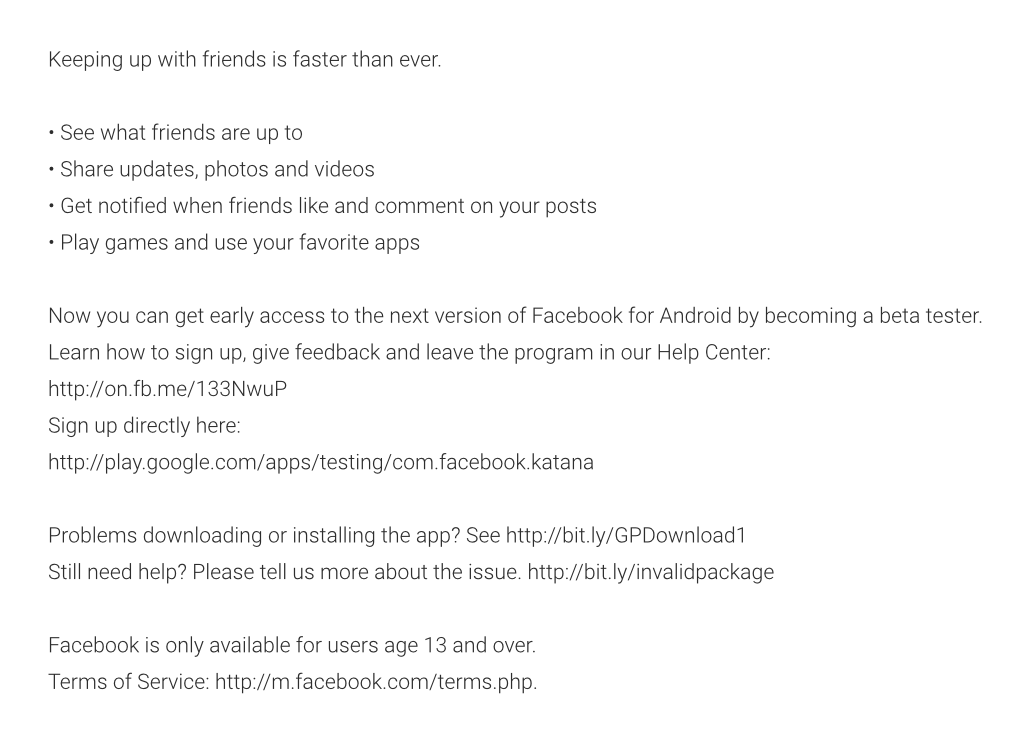
\includegraphics[width=4.7in]{figures/fb_desc}
	\caption{Facebook移动应用描述信息。}
\end{figure}

由于Google Play移动应用商城通常包含多种语言,即使本文以英文为主要研究对象语言,但其中依旧会夹杂其他语言的文字。例如,有些开发者会在发布的移动应用的英文描述最后,加上一两句用开发者本国语言写的相关介绍。该做法通常是为了吸引更多本土用户,也包含其他原因。由于本文研究的问题和方法以英文为对象,因此需要将这些非英语的文字去除。本文利用自然语言处理工具Natural Language Toolkit (NLTK)\cite{nltk}将描述中的非英语部分过滤掉。此外,从图4-2可以观察到,描述文本中通常还会有标点符号、网络链接地址(例如,\texttt{http://on.fb.me/133NwuP})等,同样需要将这些无关信息过滤掉,避免影响后续特征提取。过滤后的描述文本一般只剩下英文单词,图4-3显示了对Facebook移动应用描述过滤后的结果。

\begin{figure}
	\centering
	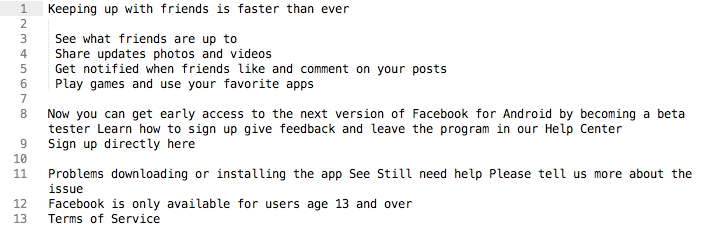
\includegraphics[width=4.7in]{figures/desc_filter}
	\caption{过滤后的Facebook移动应用描述文本。}
\end{figure}

在对描述文本进行过滤操作后,为了抓取文本中最关键的单词,从而理解文本语义信息,本文将描述文本中无关紧要的停用词去除并提取词干。停用词是语言中最常出现的助词、介词、连词等一些单词,其本身不具有特别意义,例如英文中的“the”、“at”、“which”等。本文利用一个停用词列表,将这些并不含有实际意义的单词去除。在去除停用词后,本文需要对描述本文进行词干提取。词干提取是自然语言处理中通用的方法,用以识别单词的词根形式,减少文本中的单词数量。例如,单词“stems”、“stemmer”、“stemming”、“stemmed”都是基于单词“stem”变化形式生成的,因此“stem”是这些单词的词根。由于这些单词虽然在形式上不同,但是其实际语义并无差异,因而在自然语言处理中将这些单词都转化成同一词根表现形式,以减少文本中不同单词的数量,从而提高特征提取效率。在对Facebook移动应用的描述文本进行停用词去除和词干提取后,其最终结果如图4-4所示。

\begin{figure}
	\centering
	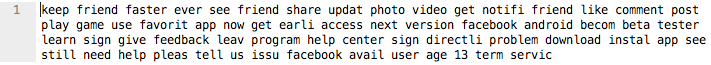
\includegraphics[width=4.7in]{figures/desc_stem}
	\caption{去除停用词并提取词干后的Facebook移动应用描述文本。}
\end{figure}

至此,通过对移动应用描述文本数据的清洗,本文得到了内容更为精简的文本,文本包含了移动应用的功能信息,为下一节特征的抽取做好基础准备。


\subsection{特征抽取}
在上一节描述文本的基础上,本节对描述文本中的文字进行抽象化,提取能够表征文本信息的特征向量。本文使用由Le等提出的Distributed Memory Model of Paragraph Vectors (PV-DM)模型\cite{le2014distributed}(通称doc2vec模型,本文也将采用此名称),将描述的文本内容转化成向量的形式。Doc2vec模型是基于word2vec模型\cite{mikolov2013efficient},通过加入段落向量进行扩充实现的。因此,本文将首先阐述word2vec模型的原理和过程,再在此基础上解释doc2vec模型的原理,最后阐述从移动应用描述中抽取特征的过程。

在自然语言处理研究中,经常需要对单词进行数学表示,称为词向量。通常的表示方法为,单词存在则为1,不存在就为0,这种表示方法被称为one-hot representation。然而,这种表示方法有个极大的缺陷,即词向量中数据极为稀疏。例如,一篇文章有1000个单词,那么每个词向量中只有一个维度的值为1,而其他999个维度都为0值,这对于自然语言处理而言带来了极大的困难。为了解决高维且稀疏的表示问题,研究者将向量低维化实数化,即用维度较少的实数而非高维的布尔值来表示词向量,该表示方法被称为distributed representation。因此,便有了接下来的研究问题——如何将文章中的单词表示成一个低维的实数向量?因为不同于one-hot representation表示方式,distributed representation的词向量无法直接从文章中获得。Mikolov等\cite{mikolov2013efficient}为了解决该问题,借鉴深度学习的思想和方法,提出了word2vec模型。该模型可以高效地学习生成distributed representation的词向量。Word2vec模型分为两种不同实现方式的模型:Continuous Bag-of-Words Model (CBOW)和Continuous Skip-gram Model (Skip-gram)。此两种模型的理论基础相似,只是对调了输入和输出部分。PV-DM模型是由CBOW模型演化而来,因此本文着重阐述CBOW模型(为便于阐述,下文中统一用word2vec来表示)。

Word2vec模型的目标是根据文本中的上下文来预测一个单词。如图4-5所示,word2vec模型是一个三层的神经网络结构,包括输入层、映射层和输出层。输入层由上下文的单词组成。训练伊始,word2vec会使用一个大小适当的移动窗口来抽取单词,该窗口中的单词则处于同一个语境中。若需要对单词$\mathsf{Word_t}$进行学习,那么在该单词前面的其他单词(如$\mathsf{Word_{t-2}}$、$\mathsf{Word_{t-1}}$)则为上文,后面的其他单词(如$\mathsf{Word_{t+1}}$、$\mathsf{Word_{t+2}}$)则为下文,这样便构成了局部的上下文语境。每一个单词都会被映射到一个唯一的词向量,表示为单词矩阵$\mathbf{W}$中的一列,而矩阵中列的下标对应于单词在语料库中的位置。后一层网络,不同于前馈神经网络语言模型(NNLM: Feedforward Neural Net Language Model)\cite{bengio2003neural},word2vec删去了NNLM中非线性的隐藏层,与之替换的是一个由所有单词共享的映射层。因为在神经网络的训练过程中,非线性的隐藏层通常是最复杂最耗时的结构部分,所以word2vec通过简化该部分结构,
\begin{figure}
	\centering
	\includegraphics[width=5.5in]{figures/word2vec}
	\caption{Word2vec模型结构图。}
\end{figure}
从而提高计算效率。Word2vec中的映射层其实是一个上下文词向量整合的过程,通常的操作可以是向量级联(concatenation)或者向量求和(sum)。设单词$\mathsf{Word_t}$用词向量$\mathbf{w}_t$表示,则图4-5中的映射层向量可以表示为:
\begin{equation}
concatenation: \mathbf{w}_p = \mathbf{w}_{t-2} \cup \mathbf{w}_{t-1} \cup \mathbf{w}_{t+1} \cup \mathbf{w}_{t+2}
\end{equation}
\begin{equation}
sum: \mathbf{w}_p = \sum_{\substack{i=t-2 \\ i \neq t}}^{t+2} \mathbf{w}_i
\end{equation}
其中,$\mathbf{w}_p$表示映射后的向量。最后一层是将前一层的映射向量作为特征,构建一个对数线性分类器,即根据输入的特征来对语料库中的单词进行分类,而训练过程即是学习正确分类目标单词的过程。具体的,给定需要训练的单词序列$\{\mathbf{w}_1, \mathbf{w}_2, \mathbf{w}_3, ..., \mathbf{w}_T\}$,word2vec的目标函数即为最大化以下平均对数概率:
\begin{equation}
\frac{1}{T} \sum_{t=k}^{T-k} \log p(\mathbf{w}_t \mid \mathbf{w}_{t-k}, ..., \mathbf{w}_{t+k})
\end{equation}
其中,$T$表示需要训练的单词数量,$p(\cdot)$为单词$\mathbf{w}_t$出现的条件概率值。因此,经过以上对语料库的训练,在预测过程中,只需计算目标单词在所处上下文中的条件概率值,即可得到对应的结果。通常预测的方法是使用例如softmax\cite{christopher2006pattern}这样的多分类器来实现,具体如下:
\begin{equation}
p(\mathbf{w}_t \mid \mathbf{w}_{t-k}, ..., \mathbf{w}_{t+k}) = \frac{e^{y_{\mathbf{w}_t}}}{\sum_i e^{y_i}}
\end{equation}
其中,$y_i$表示输出单词$i$未归一化的对数概率值,其计算方法如下:
\begin{equation}
y = \mathbf{U}h(\mathbf{w}_{t-k}, ..., \mathbf{w}_{t+k}; \mathbf{W}) + \mathbf{b}
\end{equation}
其中,$\mathbf{U}$和$\mathbf{b}$为softmax的参数,$h(\cdot)$是由$\mathbf{W}$中的词向量级联或求和构建而成的。为了对大量单词进行快速训练,因此在实际操作中,word2vec使用hierarchical softmax\cite{morin2005hierarchical}作为输出层的多分类器。因而,输出层实际上是一棵由Huffman树\cite{huffman1952method}构建而成的二叉树,其中每个叶子节点表示语料库中的单词,而单词在语料库中出现的次数则为其所在节点的权重,且每个节点都有唯一的编码。Word2vec对单词的训练过程使用了常见的随机梯度下降方法,梯度值是通过反向传播的方法\cite{rumerhart1986learning}进行计算的。该方法在神经网络训练中大量使用,具体算法可以参见相关文献,在此不做赘述。

\begin{figure}
	\centering
	\includegraphics[width=5.5in]{figures/doc2vec}
	\caption{Doc2vec模型结构图。}
\end{figure}

通过对word2vec模型的分析,可以发现初始随机赋值的输入词向量,在对目标单词预测的过程中,间接地转化成了富含语义的词向量。依据word2vec此特性,doc2vec于是在word2vec的基础上进行扩展,将文档作为向量加入到训练和预测的过程中。如图4-6所示,不仅来自单词矩阵$\mathbf{W}$的每一个词向量作为特征输入,而且每一个文档也被映射到一个向量(表示为文档矩阵$\mathbf{D}$中的一列)作为输入。文档向量与词向量一同作为输入,在影射层中进行级联或求和,来预测语境中的目标单词。此外,对于word2vec中公式(4-5)的$h(\cdot)$函数,将由$\mathbf{W}$中的词向量和$\mathbf{D}$中的文档向量一起构建。特别的,文档向量只在当前文档的语境中共享,即对某一文档进行训练和预测时,仅当前文档向量作为确定输入进行计算,而其他文档向量不参与计算。词向量则不同,整个词向量矩阵$\mathbf{W}$在所有文档的训练和预测中都共享使用。

本文从Google Play市场上爬取了23,398个移动应用的描述,每个描述作为表征移动应用功能的文本,经过4.3.2节的数据清洗,形成23,398个文档。这些文档作为本文实验的语料库,在此基础上进行文档向量的学习。特别的,由于移动应用的描述与日常用词不完全相同,因此本文不使用通用的词汇表对描述文档进行训练,而是利用这两万多个描述文档中出现的词汇作为实际词汇表,在训练和预测过程中作为参照。本文对每个描述文档进行长度为$l$的滑窗扫描,每个窗口中的所有单词将作为上下文语境输入模型。设描述文档矩阵为$\mathbf{T}$,其每列表示描述文档向量$\mathbf{t}_i$,则如上文所述,本文将该向量与描述文档中的每个词向量一起作为doc2vec的输入进行训练和预测。模型收敛后,本文得到一组移动应用描述文档的向量$\mathcal{T} = \{\mathbf{t}_1, \mathbf{t}_2, ..., \mathbf{t}_n\}$。获得了描述文档的向量表征后,本文将在下节中对描述向量进行相似性计算。


\subsection{相似性计算}
在推荐系统中,经常通过分析用户喜好的物品,查找与其具有相似喜好的其他用户,根据其他用户的喜好情况,为目标用户推荐可能喜好的物品。在此推荐过程中,查找相似用户是最为关键的一个步骤,因此计算不同用户间的相似情况成为推荐系统中主要部分之一。常用的相似性计算方法包括欧几里得距离、皮尔森相关系数(PCC: Pearson Correlation Coefficient)\cite{pearson1895note}、余弦相似度(Cosine Similarity)等。本文分别使用皮尔森相关系数和余弦相似度对描述文档的向量计算相似性。

\textbf{皮尔森相关系数:}皮尔森相关系数是对两个变量的线性关系的衡量。用皮尔森相关系数来表示两个移动应用的描述间的相似性,可用以下公式表示:
\begin{equation}
f_{\mathit{PCC}}(\mathbf{t}_i, \mathbf{t}_j) 
= \frac{\sum_{x=1}^\chi (t_{i,x} - \overline{t_i})(t_{j,x} - \overline{t_j})}{\sqrt{\sum_{x=1}^\chi (t_{i,x} - \overline{t_i})^2}\sqrt{\sum_{x=1}^\chi (t_{j,x} - \overline{t_j})^2}}
\end{equation}
其中,$\mathbf{t}_i$和$\mathbf{t}_j$为移动应用的描述向量,$t_{i,x}$表示描述向量$\mathbf{t}_i$中第$x$维数据,$\overline{t_i}$为描述向量$\mathbf{t}_i$各维度的均值,$\chi$是描述向量的长度。$f_{\mathit{PCC}}(\mathbf{t}_i, \mathbf{t}_j)$的取值范围在$[-1,1]$内,若$f_{\mathit{PCC}}>0$,则表示描述向量$\mathbf{t}_i$与$\mathbf{t}_j$具有正相关性;若$f_{\mathit{PCC}}=0$,则表示描述向量间没有相关性;若$f_{\mathit{PCC}}<0$,则说明是负相关。

\textbf{余弦相似度:}余弦相似度是用来衡量两个非零向量间的夹角的余弦值。用余弦相似度来表示两个移动应用的描述间的相似性,可用以下公式表示:
\begin{equation}
f_{\mathit{cos}}(\mathbf{t}_i, \mathbf{t}_j) 
= \frac{\mathbf{t}_i \cdot \mathbf{t}_j}{\parallel \mathbf{t}_i \parallel \parallel \mathbf{t}_j \parallel}
= \frac{\sum_{x=1}^\chi t_{i,x}t_{j,x}}{\sqrt{\sum_{x=1}^\chi t_{i,x}^2}\sqrt{\sum_{x=1}^\chi t_{j,x}^2}}
\end{equation}
其中,$\mathbf{t}_i$和$\mathbf{t}_j$为移动应用的描述向量,$t_{i,x}$表示描述向量$\mathbf{t}_i$中第$x$维数据,$\chi$是描述向量的长度。与皮尔森相关系数相同,$f_{\mathit{cos}}(\mathbf{t}_i, \mathbf{t}_j)$的取值范围也在$[-1,1]$内,且当$f_{\mathit{cos}}>0$时,描述向量$\mathbf{t}_i$与$\mathbf{t}_j$呈现正相关性;当$f_{\mathit{cos}}<0$时,描述向量$\mathbf{t}_i$与$\mathbf{t}_j$呈现负相关性;当$f_{\mathit{cos}}=0$,描述向量互不相关。

本文分别使用以上两种相似性计算方法对移动应用间的描述向量进行相似性计算,计算所得的结果表征了两个描述文档间的相似性,而描述文档中蕴含了移动应用的功能信息,则该相似性进而表征了移动应用间的相似程度。在第五章的实验部分,本文将详细阐述这两种相似性计算方法在第三方库推荐中的表现,并讨论他们各自的优劣。



%%%%%%%%%%%%%%%%%%%%%%%%%%%%%%%%%%%%%%%
%--------------------------------------     视图相似性     --------------------------------------%
%%%%%%%%%%%%%%%%%%%%%%%%%%%%%%%%%%%%%%%
\section{视图相似性}
经常会有不同的移动应用包含类似的功能,由于移动应用市场上充斥着大量相似的移动应用,导致开发者间的竞争异常激烈。对于相似移动应用的检测,已有较多相关的研究工作,例如利用代码克隆分析技术,将原移动应用的用户和广告收益导流到其他移动应用\cite{gibler2013adrob},或用以检测Android平台上的恶意移动应用\cite{zhou2012dissecting}。大多数已有的相似移动应用检测的方法通常是通过对反编译后的源代码分析来实现的,但此类方法具有一个缺陷——如果对移动应用的源代码进行代码混淆操作,将可能无法识别反编译后的程序代码。Chen等\cite{chen2015simapp}充分利用了移动应用市场上的各种元数据,通过两个阶段对相似移动应用进行检测,但是作者忽略了移动应用内部的信息——程序代码所包含的信息。这些算法在解决相似移动应用检测问题上都具有一定的缺陷。基于程序代码分析的方法会受到代码混淆技术的影响,且计算复杂度较高。而利用移动应用市场上元数据的方法会忽略移动应用内部所包含的功能信息。为了解决这一问题,本文从移动应用视图的角度来计算相似性,从而能够全面掌握移动应用的功能信息。


\subsection{逆向工程}
为从移动应用的视图角度对其进行分析,需要先解析移动应用的程序包。Android移动应用的程序代码编译后以\texttt{.apk}方式打包,
\begin{figure}
	\centering
	\includegraphics[width=6in]{figures/sogou}
	\caption{对搜狗输入法反编译后的程序层次结构,源代码存储在\texttt{.smali}文件中。}
\end{figure}
\begin{figure}
	\centering
	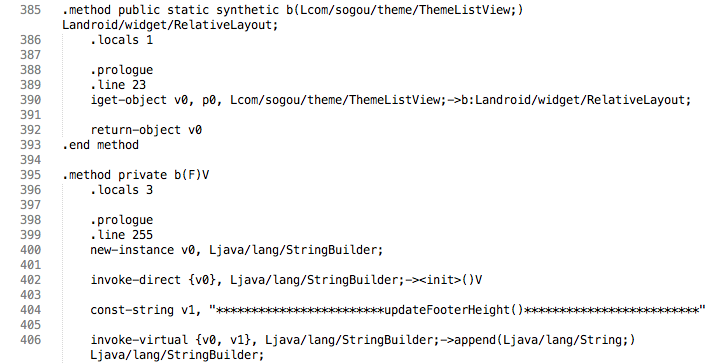
\includegraphics[width=5in]{figures/smali}
	\caption{搜狗输入法中\texttt{ThemeListView.smali}文件的部分代码。}
\end{figure}
因此需要将\texttt{.apk}程序包反编译,转化成可读的程序代码,该过程通常被称为逆向工程(Reverse Enigneering)\cite{chikofsky1990reverse}。通过逆向工程,可以对移动应用的源代码进行静态程序分析,获取内部功能信息。本文使用\textit{Apktool}\cite{apktool}工具对移动应用进行反编译操作,可以恢复移动应用中的程序层次结构。以搜狗输入法移动应用为例,反编译后的程序层次结构如图4-7所示,上方最左侧是搜狗输入法的根目录——程序包名\texttt{com.sohu.inputmethod.sogou},左侧第二列是第一级目录中的文件内容,其中\texttt{AndroidManifest.xml}是4.4.2节permissions特征存放的位置,\texttt{assets}文件夹包含了assets资源文件,\texttt{res}文件夹包含了resources资源文件。所有反编译后的程序源代码都存放在\texttt{smali}文件夹下,且以\texttt{.smali}的文件格式存储。图4-8展示了搜狗输入法\texttt{ThemeListView.smali}文件中的部分源代码,可以观察到,函数修饰符(\texttt{public/private})、函数参数(\texttt{Ljava/lang/String})、函数调用(\texttt{Landroid/widget/RelativeLayout},在4.4.2节中将讨论该类视图相关的函数)等都得到了恢复。利用反编译后的程序源代码,可以对移动应用进行视图和代码层面的分析,从而提取相关的功能特征,下节将详细讨论特征提取的方法。


\subsection{特征抽取}
本文基于视图的相似性计算方法,其动机来源于使用移动应用过程中的观察和发现。通常,人们仅仅通过查看移动应用的截图界面就能够快速辨别出两个移动应用是否相似。Viennot等\cite{viennot2014measurement}也曾提及过类似的观点。因此,本文将从移动应用视图的角度,分析其特征信息,下文将详细阐述视图特征提取过程。

\begin{figure}
	\centering
	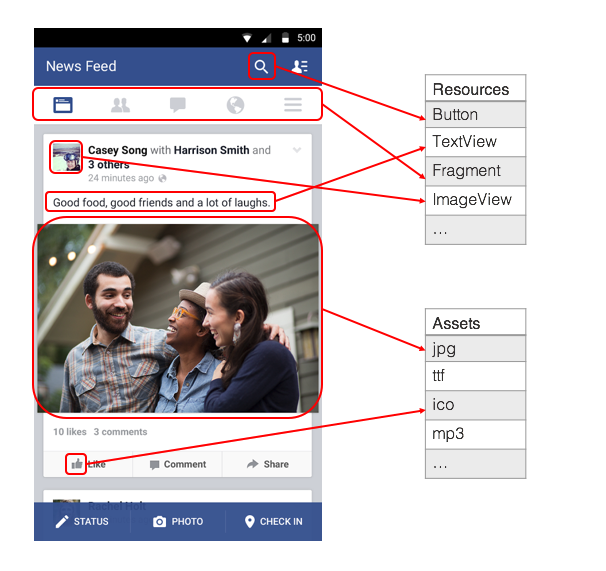
\includegraphics[width=5in]{figures/screenshot}
	\caption{Facebook移动应用中的resources和assets。左侧图片上的红色框表示Facebook移动应用所使用的resources和assets,右侧是其对应的具体列表。}
\end{figure}

在Android移动应用中,有两种主要的数据资源,分别为resources和assets。这两个数据资源存储了移动应用的视图信息,例如用户界面布局、图片、头像等。以Facebook移动应用为例,如图4-9所示,左侧部分是Facebook移动应用的用户界面,右侧则表示该移动应用中所使用的两种资源的列表。用户界面上标记的红色方框,且与右侧列表相连的列表,是Facebook移动应用中所使用的一些resources和assets资源。

Android平台上的resources资源以层次结构存储在称为\textbf{R}\cite{r}的Java类中。\textbf{R}文件是移动应用中存储界面布局resources资源名字(例如,\textit{Button}、\textit{EditText}、\textit{ListView}等)的一个基本文件。图4-10展示了一个\textbf{R}文件的例子,可以看到文件内存储了界面布局的resources名字以及对应的ID。这些resources名字对应了移动应用中相应的视图元素,如图4-10右侧红框中的\texttt{edit\_style1}是一个\textit{EditText}文本编辑框,\texttt{0x7f02000e}是其对应的ID。因此,本文通过\textbf{R}文件中的resources资源名,查找移动应用中使用对应资源的方法、函数等,从而识别相应的视图特征。本文使用4.4.1节中阐述的方法对移动应用进行逆向工程,然后对反编译后的程序代码进行分析,其代码形式如下:
\begin{center}
\texttt{Landroid/widget/ImageView;->setSelected(Z)}
\end{center}
\begin{figure}
	\centering
	\includegraphics[width=6.2in]{figures/R}
	\caption{移动应用中的\textbf{R}文件,其中包含了resources资源的名字和ID。右侧红框中给出了resources资源的一个例子,\texttt{edit\_style1}是一个resources资源的名字,\texttt{0x7f02000e}是该资源唯一编码的十六进制ID。}
\end{figure}
其中,代码的前半部分\texttt{android/widget/ImageView}表示对应代码所使用的类的名字,后半部分\texttt{setSelected(Z)}表示此函数的名字。此函数是由一个\textit{ImageView}的resources资源调用,因而可以据此将这一资源的使用情况作为resources特征,来表征移动应用的视图特征。因此,本文根据\textbf{R}文件中所列的所有resources资源名,对反编译后的源代码进行遍历,查找资源对应的调用函数,若调用了相应函数,则标记为1。从程序代码中识别的函数调用,将作为resources资源特征,用$\textbf{r}_i = \{r_{i,1}, r_{i,2}, ...\}$表示移动应用所使用的所有resources资源,其中$r_{i,1} \in \{0, 1\}$表示所调用的某一个resources相关的函数。

\begin{figure}
	\centering
	\includegraphics[width=3.2in]{figures/assets}
	\caption{移动应用中的assets文件夹,文件夹中包含了移动应用所有的assets资源文件,如移动应用启动界面的图片\texttt{ic\_launcher.png}。}
\end{figure}

对于移动应用中所使用的assets资源,可以从图4-11中观察到,该类资源是存储在移动应用程序包下的assets文件夹中。assets资源文件包括图片、音频、视频等,其通常会根据具体资源的内容进行命名,例如图4-11中的移动应用启动界面图片\texttt{ic\_launcher.png}。不同移动应用在使用assets资源时,在命名方式和文件格式上具有一定的相似性。因此本文利用这一特点,对assets资源文件进行分析,使用情况相近的移动应用通常表现出一定的相似性。所有静态的assets资源(本文暂时不考虑动态加载的资源数据)都包含在移动应用的程序包中,因此通过对\texttt{.apk}文件反编译后,可以从程序包中完全恢复其所使用的assets文件列表。本文将这些资源文件作为assets资源特征,用$\textbf{e}_i = \{e_{i,1}, e_{i,2}, ...\}$来表示移动应用所使用的所有assets资源,其中$e_{i,1} \in \{0, 1\}$表示所使用的某一个assets资源文件。

以上两类资源resources和assets是本文主要考虑的与移动应用视图相关的特征信息,可以用来表征移动应用视图以及程度代码层面的信息。为了充分利用移动应用程序包内的数据,本文同时对移动应用的permissions权限进行特征抽取。Permissions\cite{permission}是Android系统用以维护系统和用户安全的权限管理架构。由于移动设备不同于传统的个人计算机,其包含更多的物理资源(如全球定位系统、三轴振动仪等)和用户信息(如通讯录、银行卡密码等),恶意的移动应用可以通过获取这些资源和信息,从中获得非法利益,影响用户的正常使用和日常生活。为此,Android系统提供了permissions权限管理架构,用以管控这些敏感资源和信息,任何需要访问和使用相应资源的移动应用,需要主动向用户申请,并在\textit{AndroidManifest}文件中进行声明。开发者可以申请使用的permissions一共有152个,在Android开发者页面\cite{permission}可以查看所有可用的permissions权限。不同的移动应用会根据自身的功能,申请相应的权限。因此,移动应用所使用的permissions权限,一定程度上表征了移动应用所使用的功能信息。图4-12是某一移动应用的\textit{AndroidManifest}文件,红框中是该移动应用所申请的permissions权限。permissions权限的格式通常如下所示:
\begin{center}
\texttt{android.permission.ACCESS\_NETWORK\_STATE}
\end{center}
\begin{figure}
	\centering
	\includegraphics[width=6in]{figures/permissions}
	\caption{\textit{AndroidManifest}文件中声明了permissions权限列表,permissions在声明时的格式一致,如图中红框所示。}
\end{figure}
其中,\texttt{ACCESS\_NETWORK\_STATE}为权限的名字,该权限表示移动应用可以读取移动设备的网络状态,例如是否连接网络,连接的是蜂窝网络还是无线网络(Wi-Fi)。本文将移动应用在\textit{AndroidManifest}文件声明的permissions抽取出来,作为权限特征集合,表示为$\textbf{p}_i = \{p_{i,1}, p_{i,2}, ..., p_{i,152}\}$,其中$p_{i,1} \in \{0, 1\}$表示移动应用声明了某一permission权限。


\subsection{相似性计算}
本文在4.4.2中一共提取了三种类型的特征:resources、assets和permissions,此三类特征分别用$\textbf{r}_i$、$\textbf{e}_i$和$\textbf{p}_i$向量表示。因此,移动应用视图向量可以表示为$\textbf{v}_i = \textbf{r}_i \cup \textbf{e}_i \cup \textbf{p}_i$。由4.4.2节可知,视图向量使用了布尔值作为每一维特征表示,因此计算视图向量间的相似性即比较两个集合的相关性。Jaccard系数(Jaccard index或Jaccard similarity coefficient)通常作为计算两个样本集合间相似性和差异性的统计方法。本文使用Jaccard系数来表示两个移动应用在视图上的相似性,具体计算公式如下:
\begin{equation}
f_{\mathit{Jac}}(\textbf{v}_i, \textbf{v}_j) 
= \frac{| \textbf{v}_i \cap \textbf{v}_j |}{| \textbf{v}_i \cup \textbf{v}_j |}
= \frac{| \textbf{v}_i \cap \textbf{v}_j |}{| \textbf{v}_i | + | \textbf{v}_j | - | \textbf{v}_i \cap \textbf{v}_j |}
\end{equation}
其中,$\textbf{v}_i$和$\textbf{v}_j$为移动应用的视图向量,$|\textbf{v}_i|$表示视图向量$\textbf{v}_i$的长度。$f_{\mathit{Jac}}(\textbf{v}_i, \textbf{v}_j)$的取值范围在$[0,1]$之间,$f_{\mathit{Jac}}$的值越大,则表示两个视图向量间的相似度越高,进而说明两个移动应用的功能更为相似。

本文根据移动应用视图信息提取的特征来计算视图向量间的相似性,计算所得的结果表征了不同的移动应用在视图层面的相似性,从而体现了移动应用间的相似程度。在第五章实验部分,本文将详细讨论视图相似性在第三方库推荐中的表现。



%%%%%%%%%%%%%%%%%%%%%%%%%%%%%%%%%%%%%%%
%-----------------------------------     移动应用聚类     --------------------------------------%
%%%%%%%%%%%%%%%%%%%%%%%%%%%%%%%%%%%%%%%
\section{移动应用聚类}
当对一个数据量很大的数据集进行操作时,通常需要通过聚类的方法来减少计算量。聚类算法可以将相似的数据项聚集到一起,如此可以使后续的计算在一个簇内完成,而簇的大小通常与整体的数据集相差2-3个数量级,这将大大降低计算复杂度、缩短计算时间长度。由于互联网上拥有上百万的移动应用,如果需要通过与所有移动应用比较来寻找相似移动应用,显得极为不切实际。为此,本文利用聚类算法的特性,提前将功能相似的移动应用聚集到同一簇中,以提交相似移动应用检测的效率。本文利用在4.3节和4.4节中提出的文本和视图相似性计算方法,对移动应用间的相似程度进行计算。因为在聚类过程中可能使用文本相似性、视图相似性,或是文本与视图结合的相似性,所以在本节中统一用$f(\mathbf{a}_i, \mathbf{a}_j)$来表示相似性计算方法,具体计算方法如下所示(参数$\mu$为文本与视图相似性间的比重):
\begin{equation}
f(\mathbf{a}_i, \mathbf{a}_j) =
\left\{\begin{matrix}
f(\mathbf{t}_i, \mathbf{t}_j) & \mathrm{textual \: features}, \\
f(\mathbf{v}_i, \mathbf{v}_j) & \mathrm{view \: features}, \\
\mu * f(\mathbf{t}_i, \mathbf{t}_j) + (1-\mu) * f(\mathbf{v}_i, \mathbf{v}_j) & \mathrm{textual \& view \: features}.
\end{matrix}\right.
\end{equation}

K-means算法\cite{hartigan1979algorithm}是最为常见的聚类算法之一,在计算机视觉\cite{ray1999determination}、自然语言处理\cite{lin2009phrase}、地质统计学\cite{honarkhah2010stochastic}等领域被广泛应用。K-means聚类算法的目标是将$n$个观察对象划分成$k$个簇,使得每个簇内的点与中心点的平均距离最小。在本文研究的对象中,移动应用间的相似性表征了互相间的距离,这与原始的k-means算法中点与点之间的距离类似。K-means算法的目标函数是最小化每个簇内点到中心点距离的总和,即在每个簇中,需要计算簇中心点到簇内其他点的距离,中心点可以是数据集中的点,也可以是计算所得且不在数据集中的中心位置。由于本文研究的对象是移动应用,在聚类过程中,中心点必须为实际存在的移动应用,因此需要对k-means算法的目标函数做一定的调整。本文以每个簇内所有移动应用与中心移动应用间的平均相似性作为簇的相似性,对移动应用进行聚类,平均相似性的计算公式如下所示:
\begin{equation}
\mathit{Sim} = \frac{1}{m} \sum_{\mathbf{a}_o, \mathbf{a}_i \in S} f(\mathbf{a}_o, \mathbf{a}_i)
\end{equation}
其中,$m$表示簇$S$中移动应用的数量,$\mathbf{a}_o$表示簇$S$中心移动应用的特征向量,$f(\cdot)$为\textbf{定义4.1}和公式(4-9)中的移动应用相似性计算方法,根据具体的特征类别(文本或视图)来计算相应的相似性。那么,k-means的目标函数可以调整为如下形式:
\begin{equation}
\underset{\mathcal{S}}{\arg \max} \sum_{l=1}^{k} \frac{1}{m} \sum_{\mathbf{a}_o, \mathbf{a}_i \in S_l} f(\mathbf{a}_o, \mathbf{a}_i)
\end{equation}
其中,$\mathcal{S}$表示$k$个簇的集合,$S_l$为第$l$个簇。由于移动应用间的相似值越大,表示相互间的相似程度越高,因此在目标函数中需要最大化$k$个簇的相似性总和。

在原k-means算法基础上,对其目标函数进行改造,可以适用于本文研究对象的聚类问题。然而,在目标函数中使用平均相似性,只考虑了簇的中心移动应用与簇内其他移动应用间的相似性,忽略了每一对移动应用间的两两相似情况,这可能会导致聚类偏差问题——每个簇有较小的均值,方差却很大。如果出现这样的情况,则并没有实现将相似的移动应用都聚到一个簇中。如图4-13所示,现有四个移动应用,其中$\mathsf{app_1}$、$\mathsf{app_2}$和$\mathsf{app_3}$是由平均相似性聚类而成的三个移动应用簇,其中$\mathsf{app_3}$为簇的中心。从图中观察可以发现,由于$\mathsf{app_4}$与中心移动应用的相似值(红色框)要小于$\mathsf{app_1}$与中心的相似值,导致在聚类过程中,$\mathsf{app_4}$被排除在外。
\begin{figure}
	\centering
	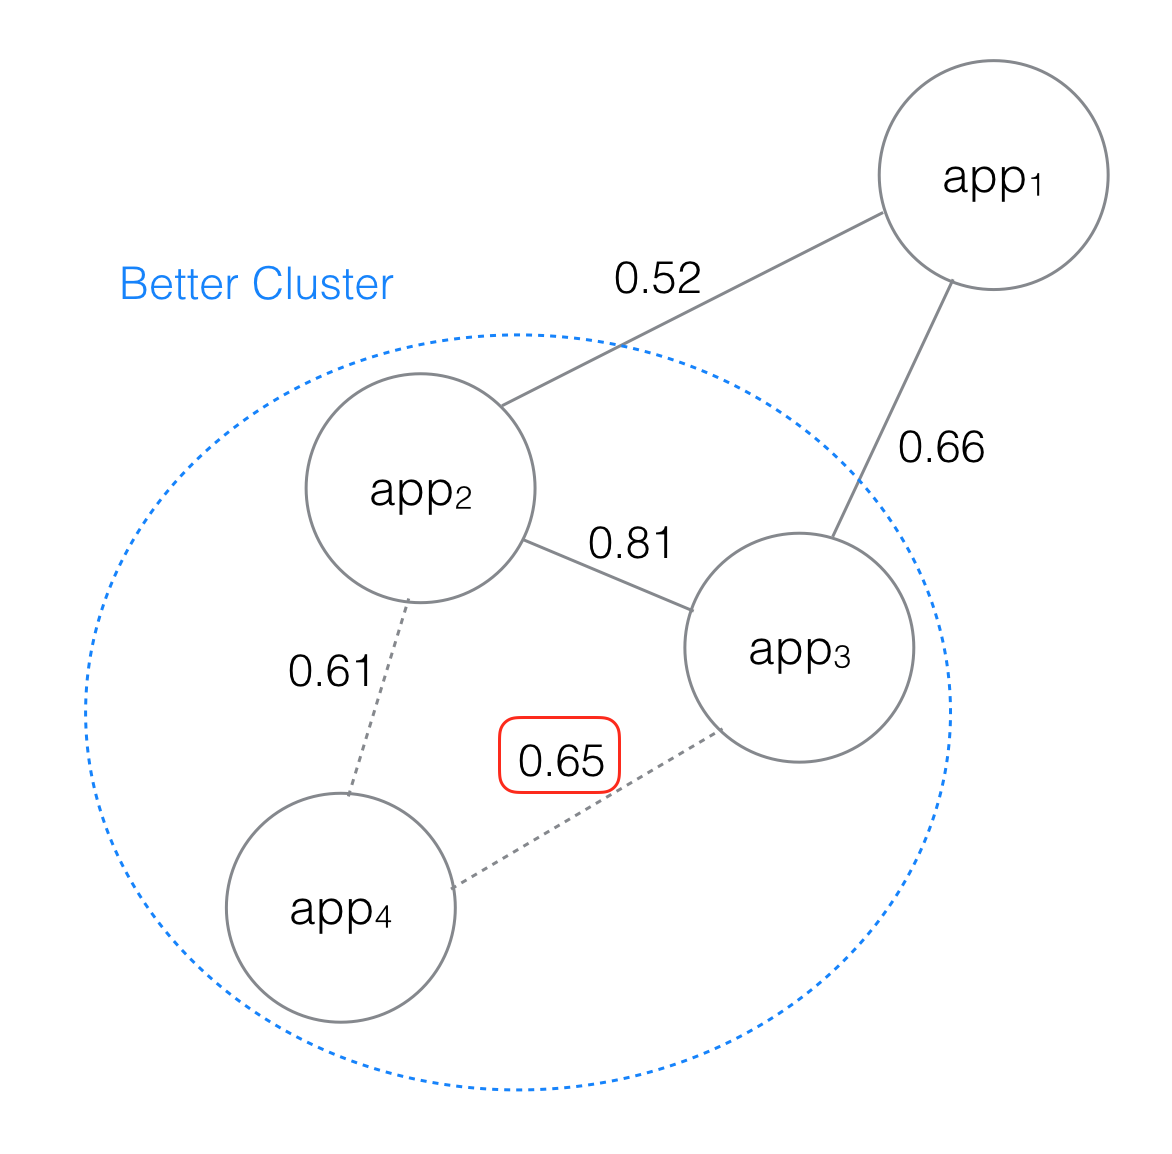
\includegraphics[width=4.8in]{figures/clustering}
	\caption{四个移动应用通过平均相似性聚类后的结果(实线连接)与可以更好的聚类结果(蓝色虚线圈)的比较。实线表示聚类后的连接关系,虚线表示可能的连接关系,连接线两侧的数据表示所连接的移动应用间的相似值。}
\end{figure}
通过观察可以发现的是,蓝色虚线圈所包括的三个移动应用,相互间更为相似。虽然$\mathsf{app_1}$被聚类在最终的簇中,但其于$\mathsf{app_2}$的相似性较其他移动应用要小得多,本不该被聚类在簇中。由于平均相似性忽略了$\mathsf{app_1}$和$\mathsf{app_2}$之间的相似性关系,导致最终的聚类结果差强人意。

凝聚式的层次聚类算法\cite{hierarchical}与k-means聚类算法不同,其将每个观察对象看作是单独的一个簇,通过不断合并距离最近的簇,最终达到聚类效果。该聚类算法考虑了观察对象之间的两两关系。其中,使用单连接法的凝聚式层次聚类,以最小距离作为聚类评判标准,将距离最小的簇合并。应用于移动应用聚类,则以最大相似性作为判别方法,具体公式如下:
\begin{equation}
\max \{ f(\mathbf{a}_x, \mathbf{a}_y) : \mathbf{a}_x \in \mathcal{X}, \mathbf{a}_y \in \mathcal{Y} \}
\end{equation}
其中,$\mathcal{X}$和$\mathcal{Y}$表示两个簇,$\mathbf{a}_x$和$\mathbf{a}_y$分别为簇$\mathcal{X}$和簇$\mathcal{Y}$内的移动应用,$f(\mathbf{a}_x, \mathbf{a}_y)$为移动应用间的相似性。从该聚类算法看,似乎可以解决k-means所遇到的问题——无法利用移动应用间的两两相似性,但实则仍具有局限性。以图4-13为例,四个移动应用初始均属于不同的簇($\{\mathsf{app_1}\}$,$\{\mathsf{app_2}\}$,$\{\mathsf{app_3}\}$,$\{\mathsf{app_4}\}$),需要计算两两相似性,将最相似的两个簇合并。使用单连接的方法进行操作,$\{\mathsf{app_2}\}$和$\{\mathsf{app_3}\}$间具有最大的相似性,因此将合并为同一个簇。此时,簇的情况为$\{\mathsf{app_1}\}$,$\{\mathsf{app_2}, \mathsf{app_3}\}$,$\{\mathsf{app_4}\}$。再次对各个簇进行两两相似性计算,使用公式(4-12)计算$\{\mathsf{app_1}\}$和$\{\mathsf{app_2}, \mathsf{app_3}\}$之间所得的值为0.66,而$\{\mathsf{app_4}\}$和$\{\mathsf{app_2}, \mathsf{app_3}\}$间的结果为0.65。显然,$\{\mathsf{app_1}\}$将会与$\{\mathsf{app_2}, \mathsf{app_3}\}$合并为一个簇,依旧无法获得最佳的聚类效果。

为了解决上述出现的问题和挑战,本文将簇内移动应用对的最小相似性作为簇的相似性表征,从而保证簇内真实的聚类情况。基于此,本文对现有的聚类算法进行优化和改进,提出了新的聚类算法,命名为k-min聚类算法。下面对k-min聚类算法进行定义:
\begin{definition}[K-min聚类算法]
给定一组移动应用$(\mathbf{a}_1, \mathbf{a}_2, ..., \mathbf{a}_n) \in \mathcal{A}$,其中每个移动应用为$\mathbf{a}_i = \{\mathbf{t}_i, \mathbf{v}_i\}$包含文本或视图的向量,k-min聚类算法的目标是将这$n$个移动应用分成$k(\leq n)$个簇$\mathcal{S} = \{S_1, S_2, ..., S_k\}$,且最大化移动应用对的相似性的最小值,即最优化以下目标函数:
\begin{equation}
\underset{\mathcal{S}}{\arg \max} \sum_{l=1}^{k} \mathcal{F}_l,
\end{equation}
\begin{equation}
\mathcal{F}_l = \min_{\mathbf{a}_i, \mathbf{a}_j \in S_l} f(\mathbf{a}_i, \mathbf{a}_j)
\end{equation}
其中,$\mathcal{F}_l$是簇$S_l$的相似值,$f(\mathbf{a}_i, \mathbf{a}_j)$为\textbf{定义4.1}中的相似性计算函数。
\end{definition}

本文提出的k-min聚类算法是用以对相似移动应用进行聚类的方法,该算法保证了每个簇都具有最大的簇内相似性和最小的簇间相似性。为了最优化\textbf{定义4.2}中的目标函数,本文引入了两个参数:参数$\varepsilon$用来控制聚类的精度,参数$\eta$用来控制迭代的次数。\textbf{算法4.1}中给出了k-min聚类算法的主要过程,包括以下四个步骤:

\begin{figure}[htb]
\centering
\begin{minipage}{.7\linewidth}
\begin{algorithm}[H]
	\small
	\caption{K-min聚类算法}
	\begin{algorithmic}[1]
	\Require
		\Statex $\mathcal{F}$ : Cluster Similarity
		\Statex $k$ : Cluster Number
		\Statex $\eta$ : Iteration Number
		\Statex $\varepsilon$ : Precision Control
	\Ensure
		\Statex $\mathcal{S}$ : Clusters
	\Statex
	\State $\mathcal{C} \leftarrow$ Random Apps
	\While {$\eta > 0$}
		\State $\Phi = True$
		\For {$i \leftarrow 1, k$}
			\State $\Delta = \mathcal{F}_i^{\eta} - \mathcal{F}_i^{(\eta+1)}$
			\If {$\Delta < 0$ or $\Delta > \varepsilon$}
				\State $\Phi = False$
				\State break
			\EndIf
		\EndFor
		\If {$\Phi$}
			\State break
		\Else
			\For {$i \leftarrow 1, k$}
				\State $\mathcal{C}_i = \underset{\mathbf{a}_x, \mathbf{a}_y \in S_i}{\arg \max \min} f(\mathbf{a}_x, \mathbf{a}_y)$
			\EndFor
		\EndIf
		\State $\eta = \eta - 1$\
	\EndWhile
	\end{algorithmic}
\end{algorithm}
\end{minipage}
\end{figure}

\begin{itemize}
\item
步骤1(1-3行):从移动应用集合$\mathcal{A}$中随机筛选出$k$个移动应用作为$k$个簇的初始中心移动应用。参数$\Phi$用以检查每次迭代后的结果,具体如下:
\begin{equation}
\Phi =
\left\{\begin{matrix}
True & \Delta > 0 \, \& \, \Delta < \varepsilon, \\
False & \mathrm{otherwise}.
\end{matrix}\right.
\end{equation}
其中,参数$\Delta$表示每次迭代后各簇相似性的变化情况,参数$\varepsilon$用以控制聚类算法的精度。本文将参数$\Phi$初始化为\textit{True};

\item
步骤2(4-10行):对每一簇,计算簇相似性的变化情况,如下:
\begin{equation}
\Delta = \mathcal{F}_l^{\eta} - \mathcal{F}_l^{(\eta+1)}
\end{equation}
其中,$\mathcal{F}_l^{(\eta+1)}$表示簇$S_l$在上一轮迭代中的簇相似性,$\mathcal{F}_l^{\eta}$则为当前轮迭代中的簇相似性。如果两轮迭代间簇相似性的差值小于参数$\varepsilon$的话,则聚类算法将结束;

\item
步骤3(11-17行):如果在新一轮的迭代中,簇相似性未发生大的变化,则算法将结束;不然,将对当前轮的各簇进行更新。具体而言,对当前轮迭代中的各簇,重新选择簇的中心移动应用,使得中心移动应用与簇内其他移动应用相似性的最小值最大化,具体公式如下:
\begin{equation}
\mathcal{C}_i = \underset{\mathbf{a}_x, \mathbf{a}_y \in S_i}{\arg \max \min} f(\mathbf{a}_x, \mathbf{a}_y)
\end{equation}
其中,$\mathcal{C}_i$为簇$S_i$的中心移动应用。对簇内任一移动应用$\mathbf{a}_x$而言,与其相似性最小的移动应用$\mathbf{a}_y$表征了移动应用$\mathbf{a}_x$所在范围(相似圈)的最边缘点,是本文最为关注的相似值。因此对这一相似值最大化,即使得移动应用$\mathbf{a}_x$相似圈最紧凑,以更小的相似半径(更大的相似值)包括簇内所有移动应用。

\item
步骤4(18-19行):对迭代参数$\eta$进行更新,从而进行下一轮的聚类迭代。
\end{itemize}

在k-min聚类算法中,参数$\varepsilon$和$\eta$用来控制聚类过程中整体的算法精度,保证能够在有限轮迭代中获得最优的聚类结果。通常而言,更大的$\varepsilon$参数和更小的$\eta$参数能够得到更好的聚类结果。根据移动应用的相似程度,对移动应用进行聚类操作,可以更快速更高效地找到与目标移动应用功能相近的其他已有移动应用,从而为后续的第三方库推荐做准备。对k-min聚类算法的表现将在第五章实验部分,与k-means和单连接的层次聚类算法进行对比实验,并详细讨论他们的优劣。



%%%%%%%%%%%%%%%%%%%%%%%%%%%%%%%%%%%%%%%
%-------------------------------------     第三方库推荐     ------------------------------------%
%%%%%%%%%%%%%%%%%%%%%%%%%%%%%%%%%%%%%%%
\section{第三方库推荐}
由于第三方库是由第三方开发者(个人或组织)开发并维护的,因此无法保证这些第三方库的质量优劣。如果移动应用开发者采用了质量较差的第三方库,不仅不能提高移动应用的用户体验,反而会减低其体验效果,甚至影响开发者声誉。为解决这一问题,则需要从移动应用开发者处收集对所使用的第三方库的反馈信息,以获取更多实际使用中可能存在的问题,为其他开发者提供参考和借鉴。本文通过分析评分较高的移动应用所使用的第三方库情况来解决这一问题。换而言之,评分较高的移动应用从其用户评分情况来看,可以认为其具有较好的质量。而分析这些质量较高的移动应用所使用的第三方库,能够相应得到质量较高的第三方库。此外,两个移动应用间的相似性显然非常重要,因为这表征了他们功能间的相似程度。

本文提出的TV-LibRec第三方库推荐算法充分利用了移动应用间的相似性,以及每个移动应用本身的质量(用户评分)。本文在4.3节和4.4节中分别讨论的移动应用文本和视图的特征,以及不同移动应用间相似性的计算方法。由以上两种相似性计算方法计算所得的移动应用具有很强的功能关联性,因此开发者采用这些相似移动应用中所使用的第三方库显得合情合理。此外,互联网上的移动应用有上百万之多,其质量良莠不齐,如果使用低质量的第三方库,则会对开发者产生不良影响。所以,需要考虑移动应用本身的质量情况,本文采用用户评分来衡量这一影响因素。因此,在为开发者推荐第三方库时,首先要根据开发者的需求寻找与之相关的相似移动应用,且同时考虑这些相似移动应用的评分情况。其次,将找到的相似移动应用中所使用的第三方库抽取出来,分析获得最为常用且质量最高的第三方库,为开发者推荐最合适的第三方库。本文在4.5节中对相似移动应用进行了聚类操作,可以基于此定位开发者的目标簇,从而使用top-z筛选方法选择与开发者期望最接近的若干个相似移动应用。本文对top-z筛选方法作如下定义:
\begin{definition}[Top-z筛选方法]
给定一组移动应用$(\mathbf{a}_1, \mathbf{a}_2, ..., \mathbf{a}_m) \in S$,top-z筛选方法的目的是从移动应用集合$S$中找到与开发者需求移动应用$\mathbf{a}_t$最相关的$z(\leq m)$个移动应用,其目标函数为:
\begin{equation}
\mathcal{L} = \{\mathbf{a}_i | i \leq z, \mathbf{a}_i \in \underset{S}{\arg sort} (D(\mathbf{a}_t, \mathbf{a}_j) | \mathbf{a}_j \in S, j \neq t)\}
\end{equation}
\begin{equation}
D(\mathbf{a}_t, \mathbf{a}_j) = \theta f(\mathbf{a}_t, \mathbf{a}_j) +  (1-\theta) d(\mathbf{a}_j)
\end{equation}
\begin{equation}
d(\mathbf{a}_j) = \frac{rating\_of\_app(\mathbf{a}_j)}{5.0}
\end{equation}
其中,函数$sort(\cdot)$将簇内的所有移动应用根据关系函数$D(\cdot)$的计算值按逆序排列。关系函数$D(\cdot)$表征了簇内移动应用与目标移动应用间的功能关系,由他们间的相似性函数$f(\cdot)$和移动应用质量$d(\cdot)$共同决定。关系函数$D(\cdot)$的值越大,则表示簇内移动应用$\mathbf{a}_j$与目标移动应用$\mathbf{a}_t$的功能关系越紧密。函数$d(\cdot)$表示移动应用的质量,用移动应用的实际评分除以最高评分五星,从而表示移动应用在用户评价中的质量表现。参数$\theta$用以权衡移动应用相似性与质量的比重。
\end{definition}

Top-z筛选方法根据与目标移动应用的关系度对簇内移动应用进行排序,从而给出了一个筛选后的移动应用候选列表。候选列表中的移动应用都具有较高的质量,且与目标移动应用相似性较高,因而从此列表移动应用中抽取的第三方库,可以推荐给开发者使用。移动应用间的相似性表征了他们之间的功能关系,亦包含了其使用的第三方库的功能信息。因为需要为开发者推荐合适的第三方库,即包含开发者所需功能的第三方库,所以需从其他移动应用所使用的第三方库中筛选出合适功能的第三方库。移动应用间的相似性一定程度上表征了这一关系,所以本文将该相似性引入第三方库筛选中。由于候选列表中的移动应用均具有较高的质量,因此在第三方库推荐过程中,本文将主要考虑移动应用相似性这一影响因子。就推荐给目标移动应用的每个候选第三方库,本文为之计算推荐分数:
\begin{equation}
\Omega = \frac{1}{z} \sum_{\substack{\mathbf{a}_i \in \mathcal{L} \\ \mathbf{a}_i \neq \mathbf{a}_t}} f(\mathbf{a}_t, \mathbf{a}_i) \cdot I
\end{equation}
其中,参数$z$为移动应用候选列表的大小,$f(\mathbf{a}_t, \mathbf{a}_i)$为目标移动应用$\mathbf{a}_t$与候选移动应用$\mathbf{a}_i$间的相似性,相似性计算方法如公式(4-9)所示。$I \in \{0,1\}$为指示参数,表示候选移动应用$\mathbf{a}_i$是否使用某一第三方库。如果$I = 0$,则表示候选移动应用未使用相应的第三方库,说明该第三方库可能不适合目标移动应用。基于此计算的推荐分数,表征了第三方库在候选移动应用中的使用率,从而说明相应第三方库的流行程度和质量。此外,本文还将移动应用的相似性加入到推荐分数计算过程,使得推荐分数$\Omega$同时具备了对第三方库功能和质量的评判,可以保证为开发者推荐的第三方库最合适且质量最高。本文引入参数$\alpha$来把控推荐过程,对于推荐分数大于$\alpha$的第三方库,将推荐给开发者。

至此,在4.5节聚类的基础上,本文充分利用了已有移动应用的功能和质量特征,从中筛选出符合开发者需求的第三方库,不仅保证了第三方库的功能性,亦考虑了第三方库的质量情况,解决了为开发者推荐优势合适的第三方库的研究问题。



%%%%%%%%%%%%%%%%%%%%%%%%%%%%%%%%%%%%%%%
%----------------------------------------     本章小结     ---------------------------------------%
%%%%%%%%%%%%%%%%%%%%%%%%%%%%%%%%%%%%%%%
\section{本章小结}
本章对本文所研究的问题——为移动应用开发者推荐优质合适的第三方库——作了具体定义,明确了本文研究问题的目标。针对本文的研究问题,本章从移动应用开发流程的两个阶段,提出了切实有效的解决方案。本文所提出的TV-LibRec算法框架一共分为了三个部分:首先,从移动应用中提取了能表征其功能的特征,并以此来计算移动应用间的相似性;然后,利用移动应用间的相似性,对功能相近的移动应用进行聚类操作;最后,在聚类后的簇中搜寻最符合开发者需求的第三方库,进而推荐给开发者使用。

本章针对移动应用相似性计算问题,分别从文本和视图两个数据层面,提出了可行的计算方法。移动应用描述信息是开发者对所开发的移动应用的功能描述文字,其包含了移动应用最基本的功能信息。因此,本文利用描述文本中的相关信息,从中提取表征移动应用功能的特征向量。本章详细介绍了本文对描述文本数据的处理过程,并阐述了doc2vec模型从文本到特征向量的转化过程。在文本特征向量的基础上,本章给出了针对文本特征的两种相似性计算方法:皮尔森相关系数和余弦相似度。本文亦从移动应用视图角度对功能特征进行抽取。本章详细阐述了针对移动应用的逆向工程方法,从而获得移动应用程序包的程序代码数据。在此基础上,本章介绍了移动应用中两种与视图相关的资源文件:resources和assets。此两类资源结合代码层数据,充分表征了移动应用的视图特征。本章同时利用了Android系统中的权限管理架构,即permissions特征,来对移动应用在敏感资源使用上的特征进行描述。综合三类移动应用内部的资源特征,本章给出了基于Jaccard系数的相似性计算方法,用以表征移动应用在视图层面的相似性。

在相似移动应用基础上,本章详细阐述了对其的聚类算法。本章首先考察了常用聚类算法k-means和单连接的层次聚类算法在本文问题上的适用性,并对其目标函数作相应调整,以适用于移动应用的聚类。本章详细分析了k-means和单连接的层次聚类算法在本文研究中的问题,并对该问题提出了相应的解决方法。为此,本章提出了一种针对移动应用聚类问题的新聚类算法k-min算法,该算法充分利用了任意两个移动应用间的相似性,从而解决了k-means和单连接的层次聚类算法在移动应用聚类过程遇到的问题和挑战。

最后,本章就本文研究问题,给出了可行的第三方库推荐算法。在相似移动应用聚类的基础上,本章针对开发者所需的目标移动应用,定位其所在的移动应用簇。推荐算法充分利用了移动应用相似性所表征的功能特征,以及移动应用评分所表征的应用质量,筛选了一个候选移动应用列表。该列表中的移动应用都具备高相似性、高质量的特点,分析并抽取其所使用的第三方库,可以确定适合开发者需求的第三方库。因此,本章将候选列表中的移动应用所使用的第三方库一一分析,并结合其相似性,计算第三方库的推荐分数。分数较高的第三方库则推荐给开发者使用。

本章对本文研究的问题作了深入分析和探讨,提出了基于文本和视图的TV-LibRec第三方库推荐算法。TV-LibRec充分利用了移动应用在文本和视图两个层次的相似性,并优化了已有的聚类算法,从而为开发者推荐优质合适的第三方库。
\chapter{实验分析与讨论}
本章将详细描述本文所使用的数据集,实验设计以及对于实验结果的评价标准。本文在第三章提出了
在网络表征算法HLE及其增量表征算法iHLE,第四章中提出了在属性网络中的表征算法SR及其增量网络场景下的表征算法iSR,本章将在数据集上进行相关的实验并与其他著名算法进行对比分析。

%%%%%%%%%%%%%%%%%%%%%%%%%%%%%%%%%%%%%%%
%----------------------------------------     数据介绍     ---------------------------------------%
%%%%%%%%%%%%%%%%%%%%%%%%%%%%%%%%%%%%%%%
\section{数据介绍}
本文利用的数据集为5个真实数据集,其中真实数据集包括2个社交媒体数据和2个引用网络数据。这4个数据集都是在线公开数据\footnote{https://linqs.soe.ucsc.edu/data}\footnote{people.tamu.edu/~xhuang/Code.html}。
\begin{itemize}
	\item \textbf{BlogCatalog}: BlogCatalog是一个社交媒体网站,用户在上面发表博客并通过相互关注建立网络,数据集选取了5196个用户节点,包含了171,743条连边。用户节点的属性信息来自用户博客的关键词描述加工处理而成,构建了8189维用户节点的属性特征,用户的分类标签是从用户自定义的兴趣爱好中选择得来的。
	
	\item \textbf{Flickr}:Flickr是一个图片分享社区,用户通过图片分享与其他用户交互,数据集以用户间的相互关注组成网络,数据集选取了7575个用户节点,包含了239,728条连边,用户节点的属性信息来源于用户的分享内容的标签(tag)信息,提取了12047维节点属性特征。用户的分类信息来源用用户加入的兴趣社区。
	
	\item \textbf{Citeseer}:Citeseer数据集是从挑选Citeseer网站上的一些文献,文献的选择过程保证对于每一篇文献都有至少被一篇文献所引用,总共选取了3312篇文章作为网络中的节点,构建了一个文献引用网络。文献的属性是来自对内容的处理得到,通过去掉停用词和选取词干的方法,剩下的3703个单词组成词库,在对文献进行处理的时候,出现次数小于10的单词去掉,根据文献中是否存在词库对应单词,将对应特征置为0/1,于是文献节点属性特征维数为3703维。根据文献本身所属主题,文献被分为六个类别:Agents,AI,DB,IR,ML和HCI。
	
	%\item \textbf{Cora}:Cora是另一个论文引用网络,主要是机器学习细分领域的论文之间的引用关系,同样在构造数据集的时候保证最后每一篇论文都有至少有一个被引用量,该数据集包含2708篇论文,在提取论文节点的属性特征时,采用方法跟Citeseer类似,通过对全部文献去掉停用词、处理词干构建词库,去掉每篇文章中的出现少10次的词,得到1433维属性特征。根据论文的内容,将论文节点分成6种:Case Based, Genetic Algorithms, Neural和Networks, Probabilistic Methods, Reinforcement Learning, Rule learning和 Theory。
	
	\item \textbf{PubMed}: PubMed是另一个论文引用网络,主要涉及的是生物领域的文献。数据集选取了19717个论文作为网络节点,不同的是,论文节点的属性特征不是0/1型,而是用文档中对应单词TF-IDF加权得到。数据集中论文根据研究主题被分成3类:Diabetes Mellitus Experimental,Diabetes Mellitus Type 1和Diabetes Mellitus Type 2。
	
\end{itemize}
关于上述数据的具体详情,见下表,另给出BlogCatalog数据集中的度分布情况。
\begin{table}
\centering
\caption{使用数据集详细统计信息}
\begin{tabular}{C{1in}C{1in}C{1in}C{1in}C{1in}}
\textbf{数据集} & \textbf{节点数} &\textbf{连边数} & \textbf{属性数}&\textbf{类别数}\\ \hline 
BlogCatalog & 5186  & 171,743 &8189&6\\
Flickr	& 7575 &239,728 & 12,047 & 9 \\
Citeseer& 3312 & 4536  &  3703 & 6 \\
%Cora & 2708 &5429 & 1433 &7 \\
PubMed & 19,717 &44,338&500 &3 \\
\hline
\end{tabular}
\end{table}

%\begin{figure}
%	\centering
%	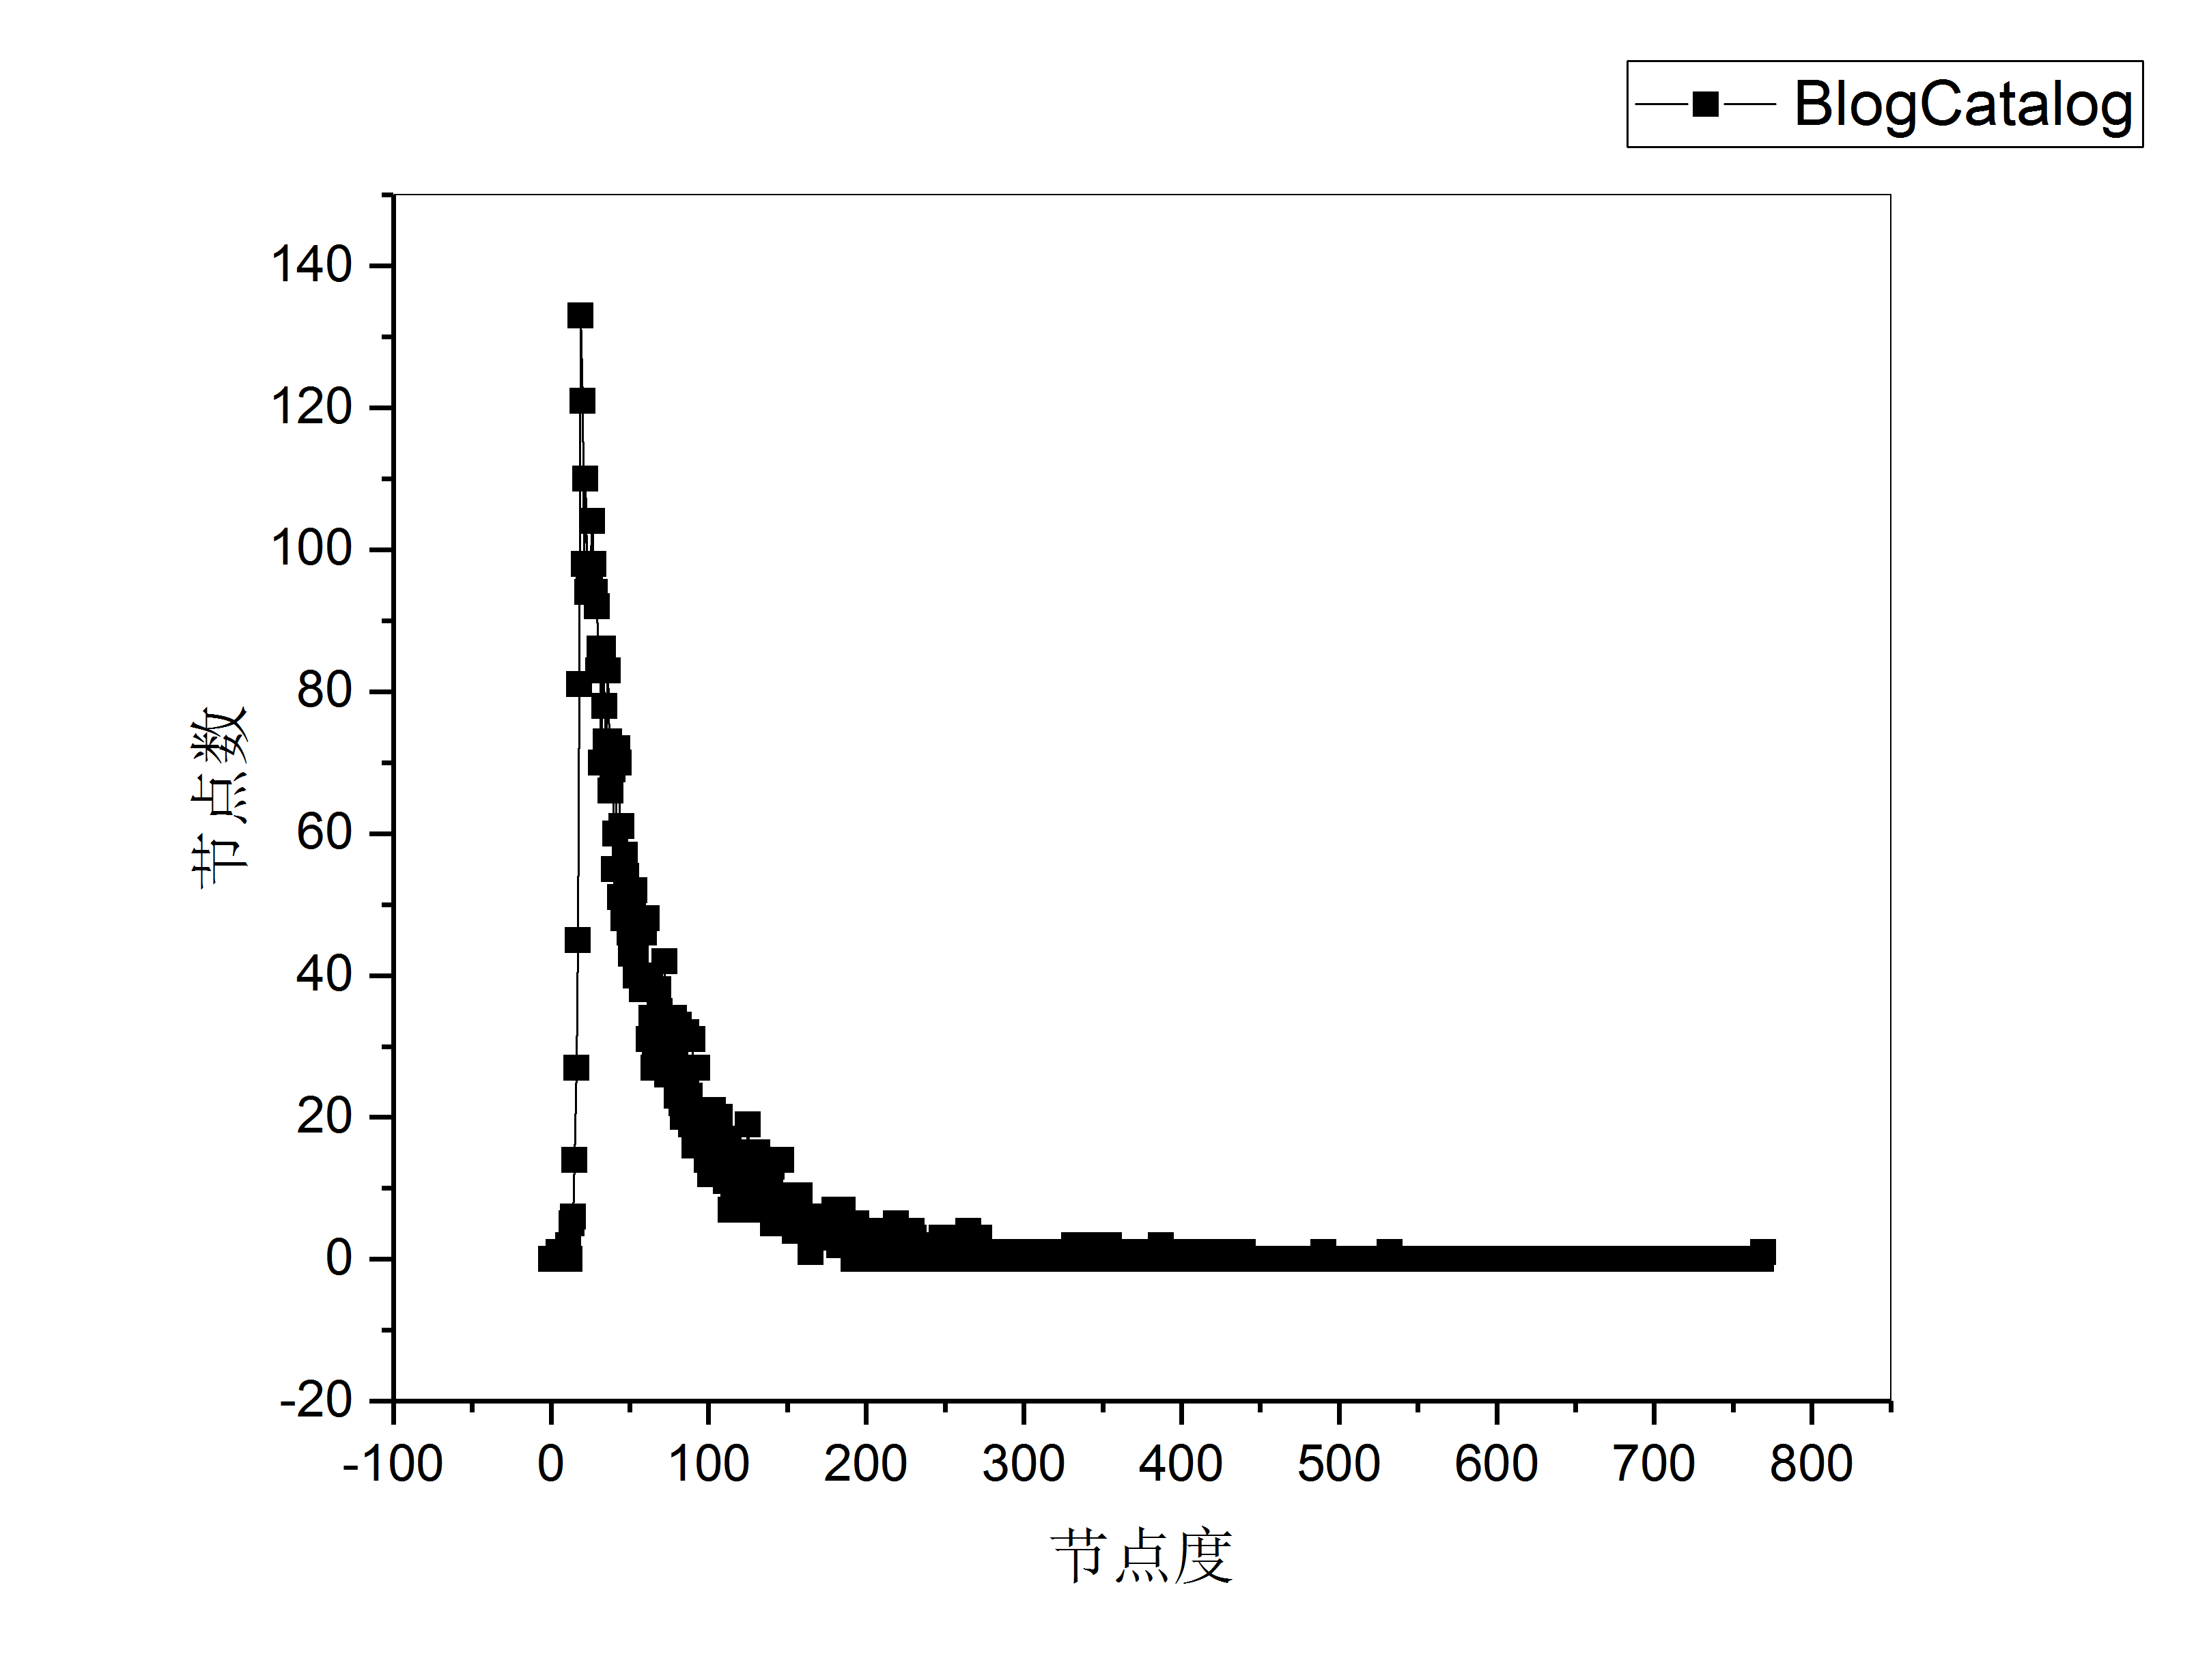
\includegraphics[width=5in]{figures/blogCatalog_degree}
%	\caption{案例数据:BlogCatalog中的度分布}
%\end{figure}
\section{实验环境}
实验的硬件环境与软件环境如表\ref{my-label5_1}所示:

\begin{table}[]
	\centering
	\caption{实验硬件与软件环境表}
	\label{my-label5_1}
	\begin{tabular}{@{}llll@{}}
		\toprule
		硬件配置\\ \midrule
		处理器&	Intel@CoreTM i7-5820k CPU @3.3GHz x 12\\ \midrule
		内存&	128G\\ \midrule
		硬盘&	1T\\ \midrule
		软件配置 \\ \midrule
		操作系统&	Ubuntu 16.04 LTS \\ \midrule
		开发环境&	Python 2.7  \\ \bottomrule
	\end{tabular}
\end{table}

\section{实验设计}
图表征算法是对网络中节点进行向量表征的过程,在这一部分主要从两方面对前面章节提出的算法进行分析评价:
\begin{itemize}
	\item \textbf{准确性}:图表征算法学习到的向量表征需要应用于后续的机器学习任务,在不同的机器学习任务中表现出来的分类预测效果如何,跟其他算法的对比效果如何?
	\item \textbf{运行效率}:基于动态增量场景提出的算法运行效率如何,跟其他离线批量算法在效率上的差异。
\end{itemize}
本节将分别从这两方面提出设计的实验过程。
\subsection{准确性评估}
在准确性评估这一部分,本章主要针对两个学习任务来进行具体的对比:一个是节点多分类任务,一个是图挖掘中常见的链路预测问题。对于不同的学习任务有不同的实验设计过程和评价准则,下面将分别对这些实验的具体过程进行介绍。

\problem{\textbf{节点多分类实验}:}节点多分类问题在一个监督学习任务,在对节点进行向量表征之后需要划分训练集和测试集,通过训练集训练模型,对测试集中的数据进行预测并评估结果的好坏。分类问题的评估方法有很多,不同于普通的二分类问题,节点分类问题是多分类过程,在节点分类任务中一般采用的评测指标有三种:分类准确率(accuracy), F1-Macro和F1-Micro。

{\textbf{衡量指标1:分类准确率}} :准确率的定义是对于给定的测试样本集,分类模型预测类别正确的样本占总样本的比例,从损失函数的角度来讲,就是模型损失函数为0-1阶梯函数时测试集上的损失值。

{\textbf{衡量指标2:F1-Macro和F1-Micro}}在介绍这两个评价准则之前,需要介绍F1值。在二分类问题中,根据实际的类别标签和预测的类别标签的不同情况可以得到混淆矩阵:
\begin{table}
	\centering
	\caption{混淆矩阵}
	\begin{tabular}{|c|c|c|c|}
		\hline
		\multirow{2}*{预测标签}& \multicolumn{2}{|c|}{真实标签} \\
		\cline{2-3}
		~ & 正例 & 反例 \\ \hline
		正例 & TP(真正例) & FP(假正例) \\ \hline
		反例 & FN(假反例) & TN(真反例) \\
		\hline
	\end{tabular}
\end{table}

其中精度P(Precision)和召回率R(Recall)可以根据混淆矩阵定义出来:
\begin{equation}
\begin{aligned}
P &= \frac{\#TP}{\#TP+\#FP} \\
R &= \frac{\#TP}{\#TP+\#FN}
\end{aligned}
\end{equation}
其中$\#\cdot$表示对应样本的个数,考虑在现实场景中精度和召回率各有不足,召回率偏向于将样本都预测为正样本,精度需要保证预测中真实正样本的比例,会偏向于将预测正样本的个数降低,F1值综合考虑精度和召回率,对两者进行统一:
\begin{equation}
	F1 = \frac{2\times P\times R}{P+R}
\end{equation}
可以看出$F1$为精度和召回率的调和平均。

在多分类问题中,无法通过二元的混淆矩阵来表示样本预测与真实之间的关系,对于$F1$因此有了在多分类情况的变形F1-macro和F1-micro。在多分类场景下需要将不同类别两两之间计算混淆矩阵,算出对应的精度和召回率,F1-macro的计算方法是:
\begin{equation}
	macro\-P = \frac{1}{n}\sum P_i
\end{equation}
\begin{equation}
macroR = \frac{1}{n}\sum R_i
\end{equation}
\begin{equation}
F1macro = \frac{2\times macroP\times macroR}{macroP+macroR}
\end{equation}
在计算完混淆矩阵后,对所有矩阵的对应值去平均得到$\overline{TP}, \overline{TN}, \overline{FN},\overline{FP}$,可以得到F1-micro的计算方法:
\begin{equation}
microP = \frac{\overline{TP}}{\overline{TP}+\overline{FP}}
\end{equation}
\begin{equation}
microR = \frac{\overline{TP}}{\overline{TP}+\overline{FN}}
\end{equation}
\begin{equation}
F1micro = \frac{2\times microP\times microR}{microP+microR}
\end{equation}
对于节点多分类问题,【本章对所有数据集进行比例抽样,从10\%到100\%对数据进行抽样,进行表征学习后,进行节点多分类任务,多分类学习任务采用逻辑斯蒂回归(Logistic Regression)算法进行学习,数据集通过5折交叉进行多次训练验证】,并通过准确率,F1-macro,F1-micro三个指标对算法效果进行评估。在对算法进行准确性评判时,分成两个部分:\textbf{离线模型}和\textbf{在线模型}。对于\textbf{离线模型}跟已有的图表征算法的效果进行对比:
\begin{itemize}
	\item 拉普拉斯特征映射算法LE:基于保留一阶接近度的图表征方法,将问题转化为求矩阵特征值的问题
	\item LINE算法:通过保留一阶接近度和二阶接近度进行图表征的算法,通过负采样优化计算。
	\item Node2vec算法:借用自然语言处理中的Word2vec思想,通过随机游走生成节点语料库,从而对图进行表征学习。
	\item CCA算法\cite{hardoon2004canonical}:将原始网络结构和原始属性特征直接作为节点分类任务的输入。
	\item AANE算法\cite{huang2017label}\footnote{https://github.com/xhuang31/AANE\_python}:将网络结构特征和属性特征同时进行优化,得到属性网络表征作为后续学习任务的输入。
	\item HLE算法:本文提出的基于高阶接近度的拉普拉斯特征映射算法。
	\item SR算法:本文提出的基于属性相似度的表征算法。
\end{itemize}
通过下面的表对实验中采用的算法进行分类:
\begin{table}
	\centering
	\caption{节点分类任务图表征算法分类}
	\begin{tabular}{|C{2in}|C{3in}|}
		\hline
		\textbf{类别} & \textbf{算法} \\ \hline 
		\multirow{4}*{网络表征}&拉普拉斯映射算法LE \\ 
		\cline{2-2}
		~ &  LINE算法	\\ 	\cline{2-2}
		~ &	 Node2Vec算法 \\ \cline{2-2}
		~ &  HLE算法	\\ \hline
		属性表征 & SR算法 \\ \hline
		\multirow{3}*{属性网络表征} & CCA算法 \\ \cline{2-2}
		~ & AANE算法 \\ \cline{2-2}
		~ & HLE+SR算法 \\ \hline
	\end{tabular}
\end{table}

\textbf{在线模型}的准确性评估实验不同于离线模型的实验设计。在离线模型评估中采用的方式为随机按比例抽样进行学习任务,不同比例的样本不存在包含关系。而在线模型中将样本分成不同的时间步,依次加入网络中进行,因此后一个时间步包含前一个时间步的样本整体。在这里需要注意的一点是,在实验过程中抽样过程先于表征算法,先完成抽样再进行表征学习,在节点分类任务时存在的训练测试集分割则在表征算法之后进行。对于在线模型,实验过程主要跟对应的离线进行准确性对比。

在对图表征算法进行准确性评判,本文还将表征向量应用于链路预测实验。
\problem{\textbf{链路预测问题}}:链路预测问题也是一个监督学习任务,但是不同于节点多分类任务的标签来源于其他附加信息,链路预测问题的标签来源于网络中的连边。链路预测问题的初衷是根据网络结构中已经存在的连边,预测没有产生连接的节点对中产生连接的概率,链路预测问题原本是基于网络对网络的学习,进一步扩展在属性网络中,利用节点本身的属性特征提高预测效果。

\textbf{属性网络中的链路预测}:给定无向属性网络$G(V,E,H)$,其中$V$代表节点集合,$E$代表连边的集合,$H$代表网络节点的属性特征集合,根据节点集合可以算出网络中所有可能连边的集合为$U$,集合的大小为$|U| = \frac{|V|(|V|-1)}{2}$,链路预测问题就是需要通过一定的算法对连边$E\prime\in U\setminus E$的可能性进行预测,也即对不存在(或未被观测到)的连边预测存在的概率。

在传统的监督学习任务中每条样本对应有特征和一个(或多个)类别标签,在模型训练之前划分训练集和测试集。本文中的链路预测也需要进行训练集和测试集的划分,在训练集中需要包含正样本和负样本,测试集也同样需要包含正负样本,正样本为在网络中确实存在的连边,也即$E$中连边,负样本连边来源于$U\setminus E$,关于训练集和测试集的划分过程如下图:
\begin{figure}
	\centering
	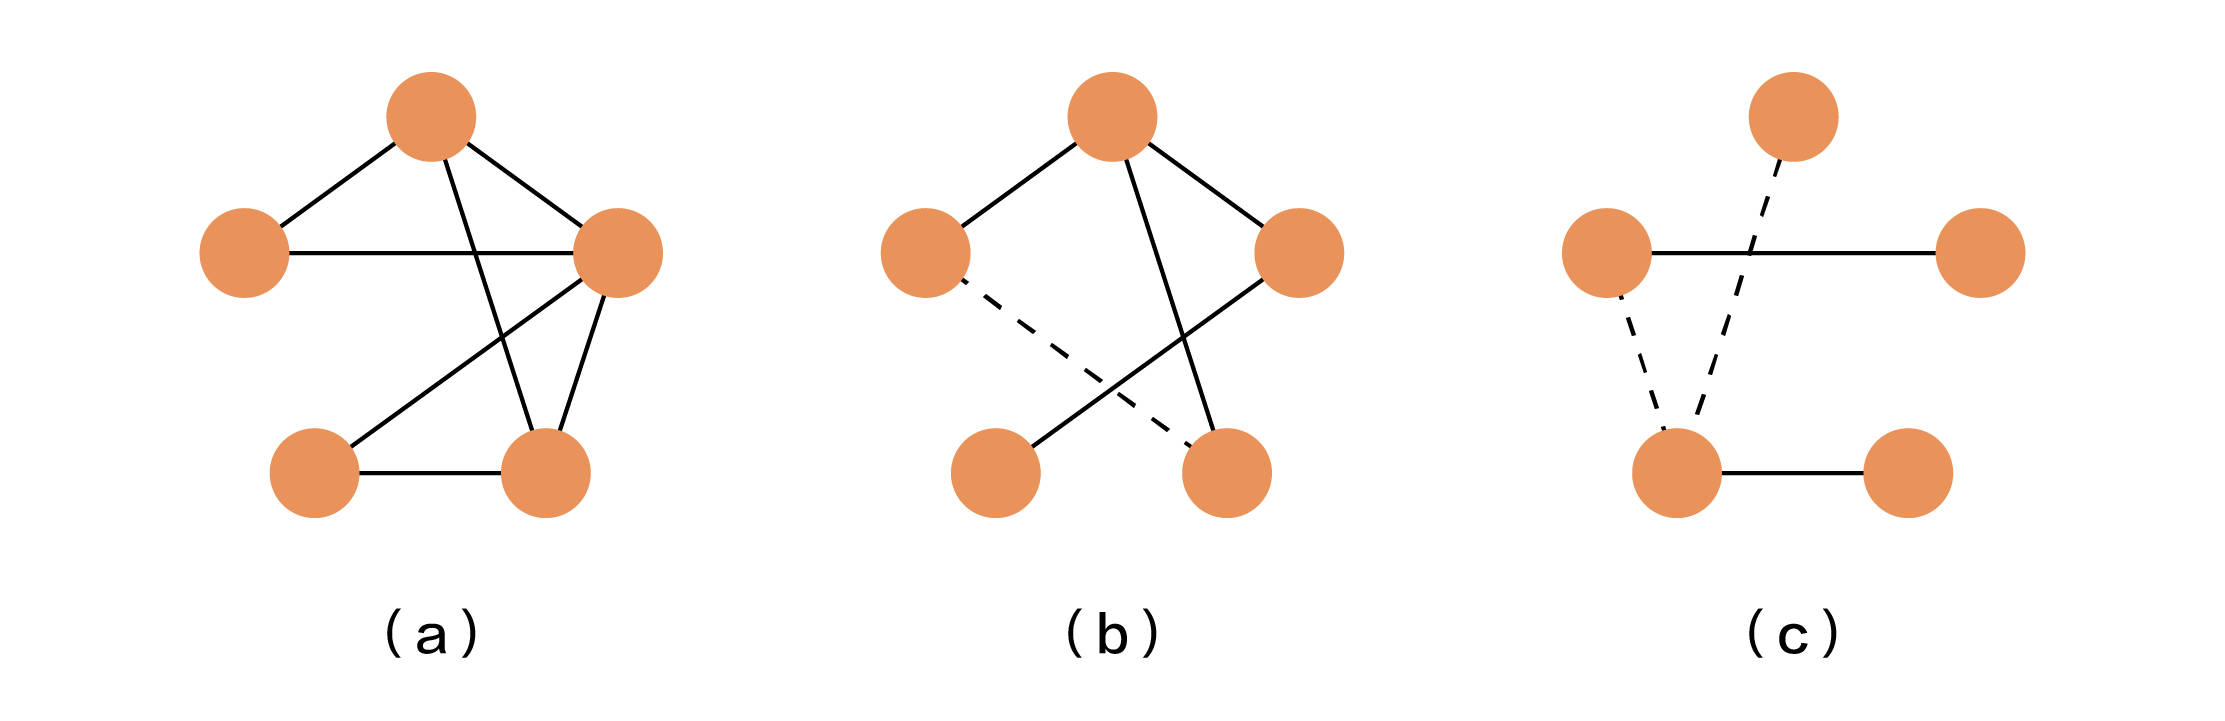
\includegraphics[width=5in]{figures/link_prediction_split}
	\caption{链路预测训练测试集划分:(a)全部连边$E$;\\(b)训练集:包含正负样本,负样本用虚线表示(c)测试集:包含正负样本}
\end{figure}

不同于上面的节点分类任务,在链路预测实验中不是直接针对节点进行k折交叉验证实验,链路预测的训练测试集是针对连边进行采样得到的,图表征算法学习到的是节点的向量表征,将图表征用于链路预测任务的直观方法是,将关于连边$e$的节点对$(i,j)$的表征向量$X_i,X_j$的函数$f(X_i, X_j)$作为该连边$e$的特征,在本文实验中采用$f(X_i, X_j) = X_i\circ X_j$ ,也即$X_i, X_j$对应元素相乘作为边的特征,再放入二分类的学习算法中,在实验中本文采用的分类算法是逻辑斯蒂回归(Logistic Regression),实验效果在测试集上进行通过\textbf{AUC}和\textbf{准确率}进行效果评价,准确率之前提及过,下面介绍一下AUC评价标准。

\textbf{衡量指标1:AUC}:AUC(Area under ROC curve),意思就是ROC(Receiver Operating Characteristic)曲线下的面积,ROC曲线是以真正例率(True Positive Rate,简称TPR)和假正例率(False Positive Rate, FPR)画出的曲线,其中以FPR为横轴,TPR为纵轴,根据混淆矩阵中的定义有:
\begin{equation}
	TPR = \frac{\#TP}{\#TP+\#FN}
\end{equation}
\begin{equation}
FPR = \frac{\#FP}{\#TN+\#FP}
\end{equation}
ROC曲线将样本按照预测概率从大到小排序,从第一个样本依次设置分类阈值为其预测值,并以此对所有样本判定预测的正负值,进一步计算出一组TPR和FPR值,以此循环可以得到一系列的值形成ROC曲线,AUC则是ROC曲线下的面积,AUC评价方法关注的是预测样本概率的排序质量。同样的,在这一部分增量学习算法主要跟对应的离线算法进行准确性对比,链路预测的实验过程图\ref{fig:link_prediction_process}所示:
\begin{figure}
	\centering
	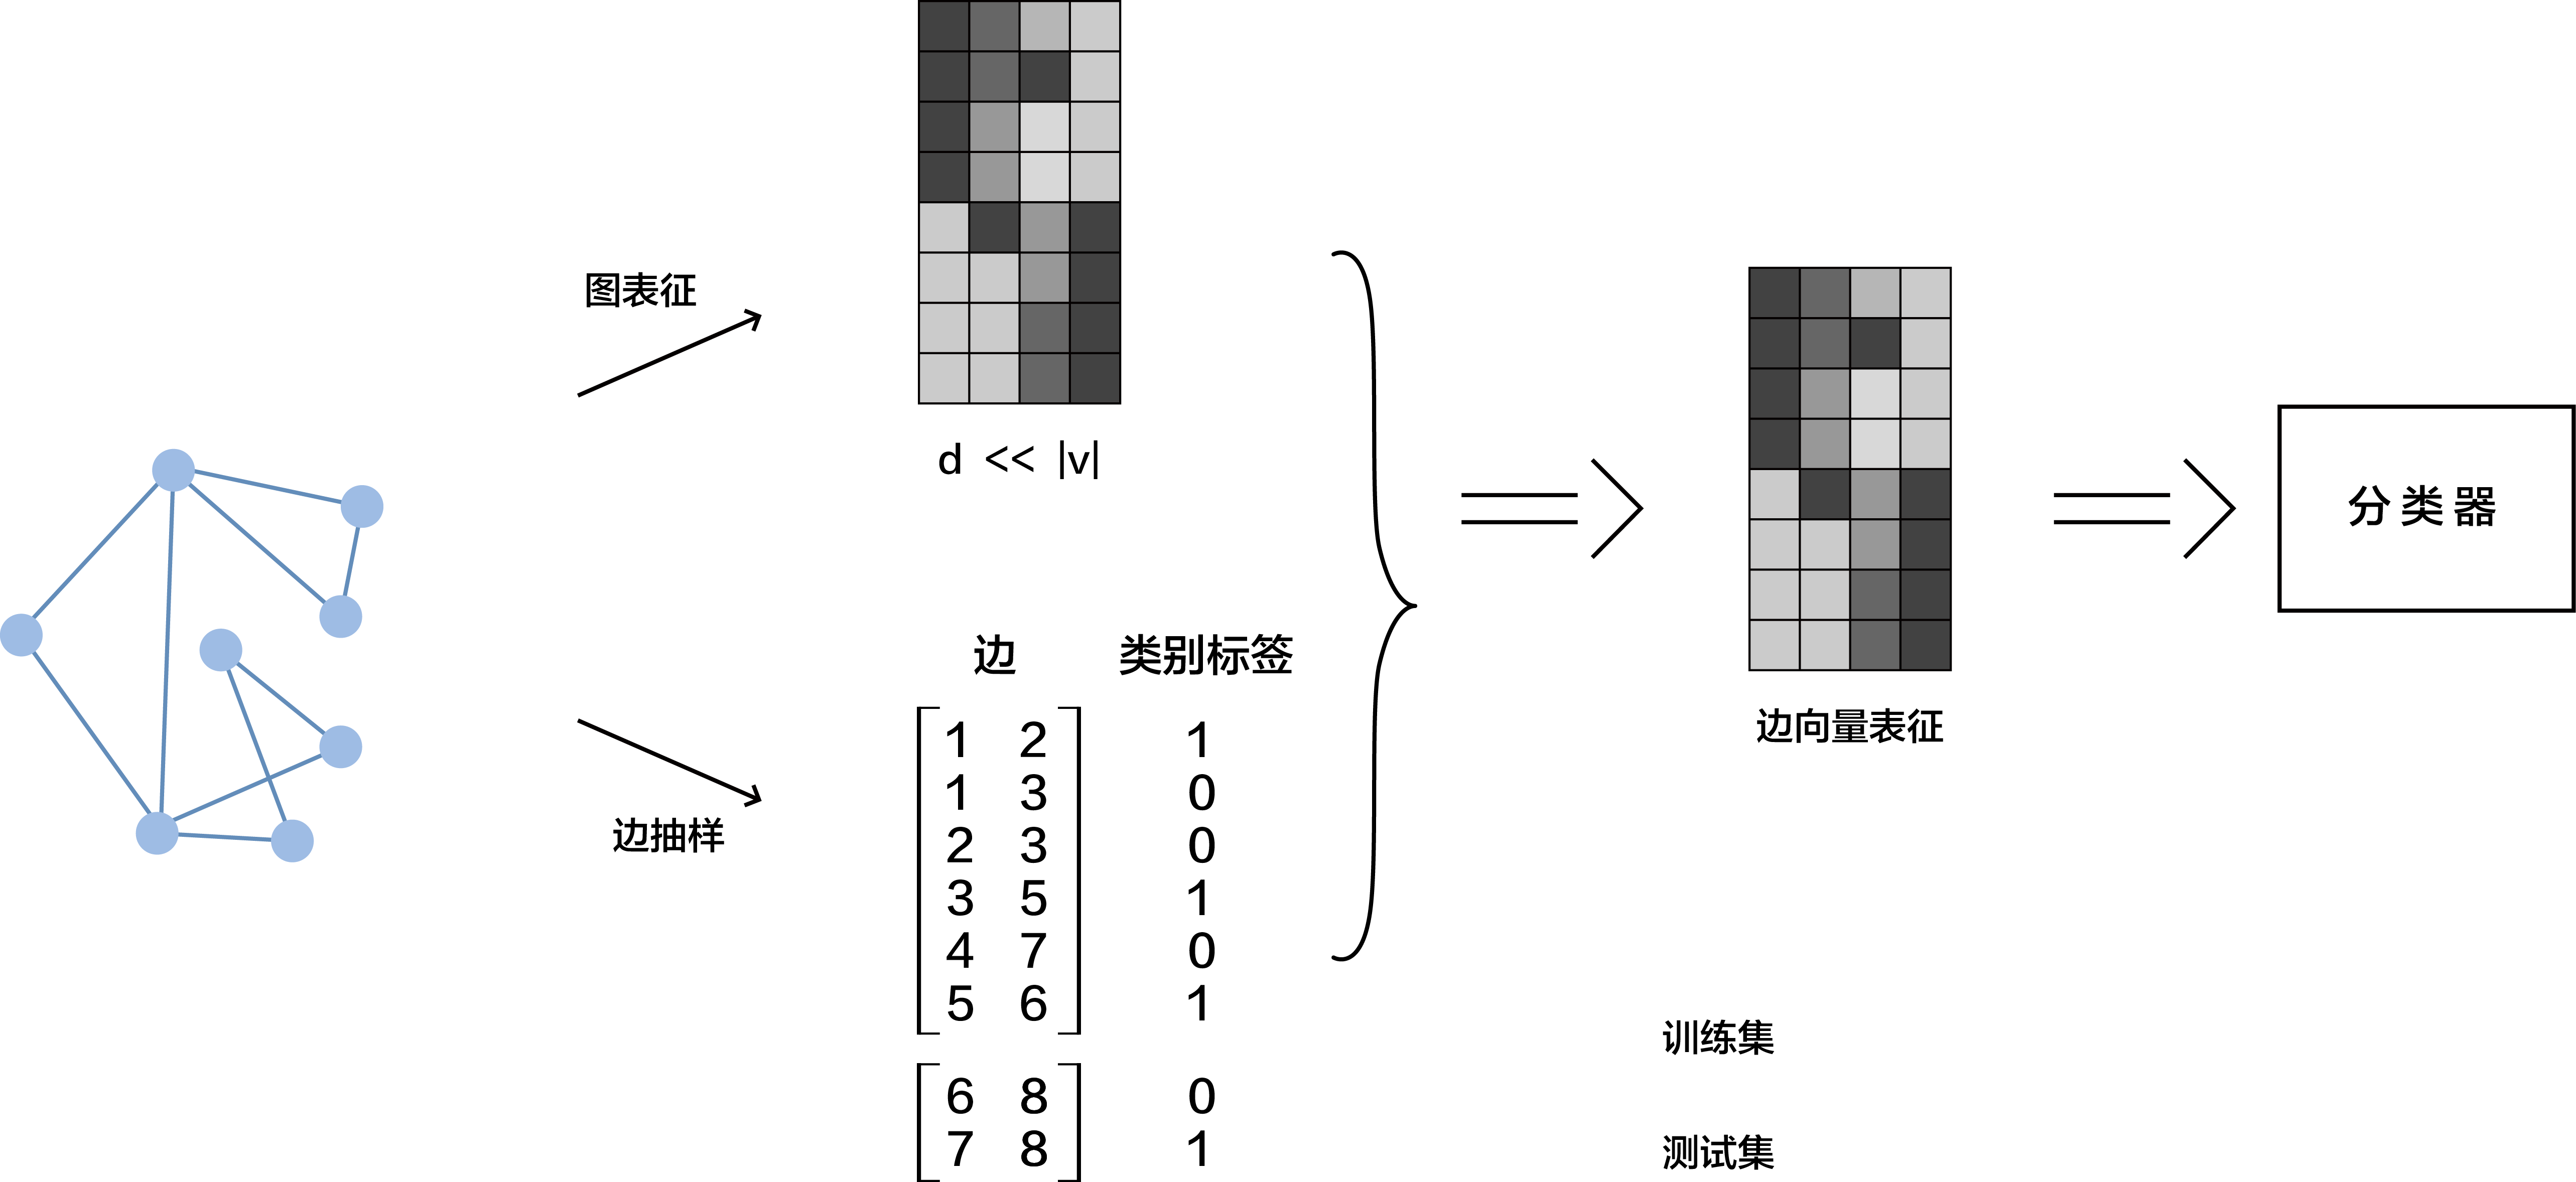
\includegraphics[width=6in]{figures/link_predict_frame}
	\caption{链路预测实验过程}
	\label{fig:link_prediction_process}
\end{figure}

\subsection{运行效率评估}
在运行效率评估这一部分,主要进行增量算法跟离线算法之间的对比,将数据集分解成多个时间步,在最初的时间步采用离线算法进行图表征,在第二个及以后时间步将分成增量算法和离线算法进行表征学习,并从两方面来对算法效果进行对比评估。
\begin{itemize}
	\item \textbf{累积运行时间}。将全部数据集分成不同时间步,计录并比较从第一个时间步到最后一个时间步之间累积所用的运行时间。
	\item \textbf{不同表征维度的效率对比}。对比在不同表征维度时,增量算法运行所有时间步所累积时间相对于离线模型的速度提升。 
\end{itemize}
\remark \textbf{关于链路预测的抽样过程}:

\remark \textbf{关于增量实验的抽样过程}:已有的数据集是一个静态的网络数据,并不包含演化过程,因此需要通过节点抽样生成一个网络演化的过程,主要思想就是通过从原有网络中逐个去掉网络中的节点,记录下过程中删除的网络节点,在增量过程中则依次加入这些节点进行表征学习,过程如图\ref{fig:network_sample}中所示:
\begin{figure}
	\centering
	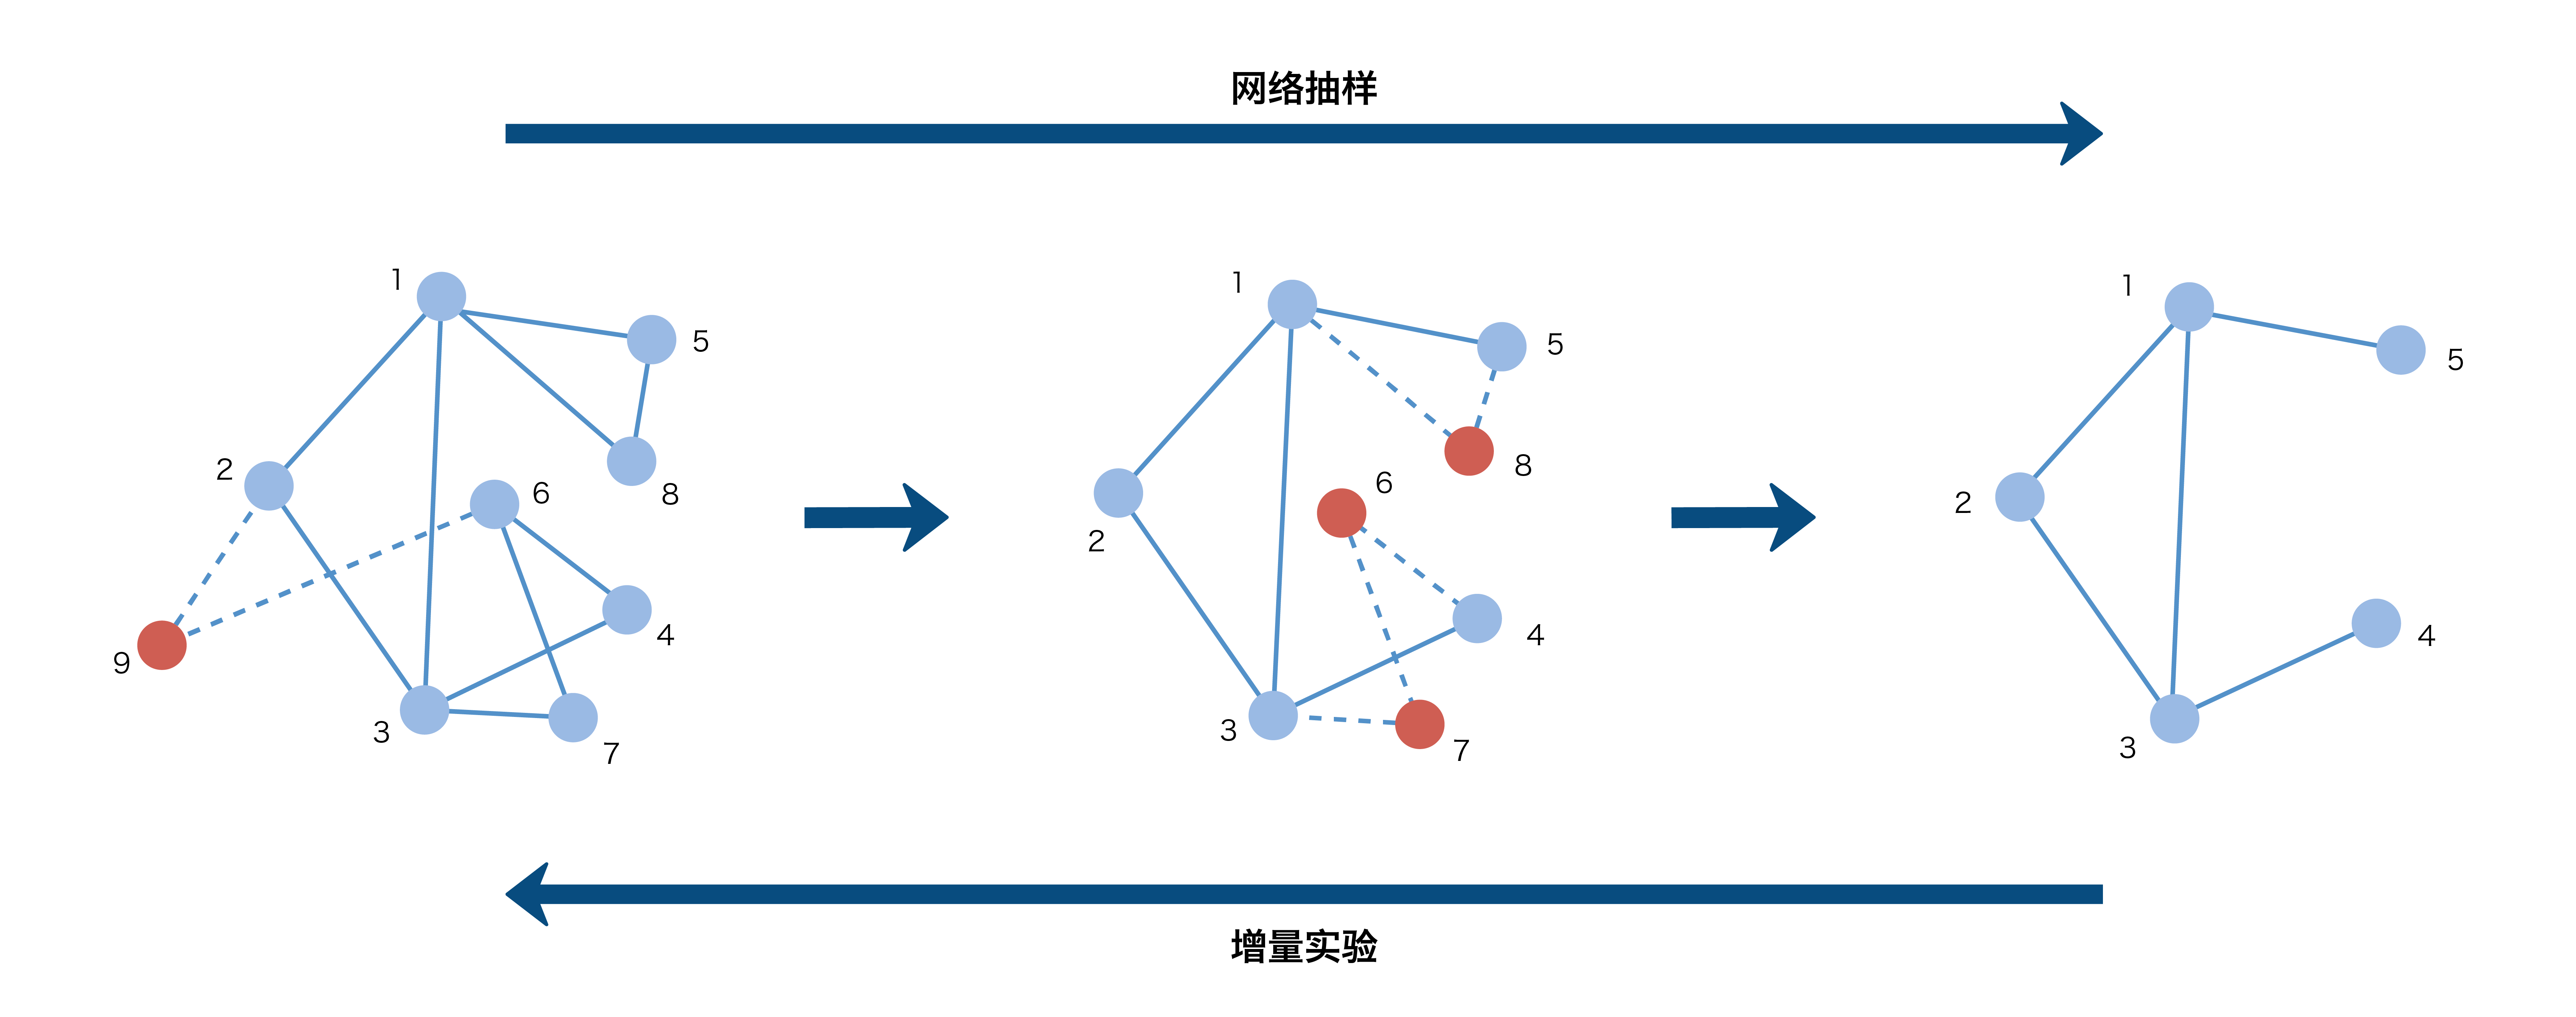
\includegraphics[width=6.2in]{figures/inc_sample}
	\caption{网络采样过程}
	\label{fig:network_sample}
\end{figure}


本文研究范围内,在网络的演化过程中,为保证节点在增量场景下进行有效表征,后加入的节点会跟先加入的节点进行连接,所以增量网络在每个时刻需要连通图的个数不能增加。反之,在抽样过程中,抽样方法需要保证删除节点前后,子图个数不会减少。在这个基本要求下,随机选取节点进行删除会存在问题,完全删除了某一个子图。因此在实验中删除节点采用启发式方式进行加速,根据节点重要性来删除,首先选择删除边缘节点,也即重要性较低的节点,在这一过程中可以通过节点度或节点Pagerank值\cite{page1999pagerank}来对重要性进行衡量,考虑到节点度的局限性,本文实验中采用节点Pagerank值来衡量节点重要性。
\begin{figure}
	\centering
	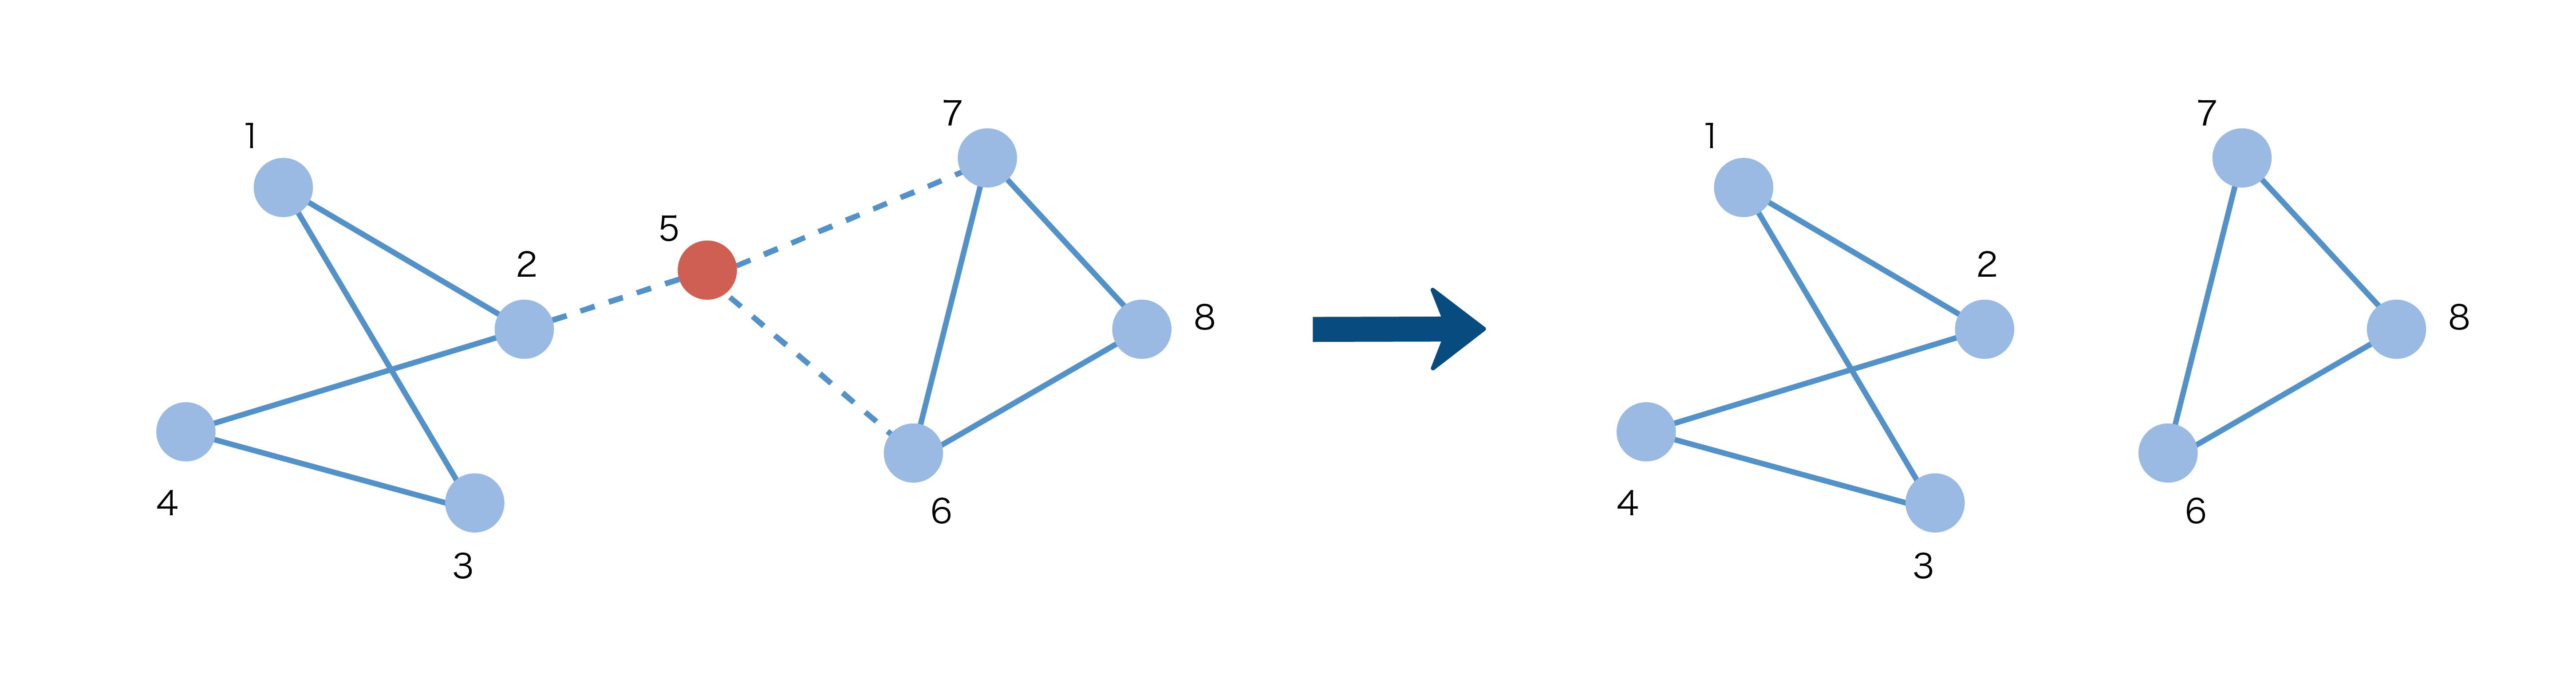
\includegraphics[width=6.2in]{figures/sample_split}
	\caption{随机采样可能出现问题}
\end{figure}


%%%%%%%%%%%%%%%%%%%%%%%%%%%%%%%%%%%%%%%
%----------------------------------------     实验结果与分析     ---------------------------------------%
%%%%%%%%%%%%%%%%%%%%%%%%%%%%%%%%%%%%%%%




%%%%%%%%%%%%%%%%%%%%%%%%%%%%%%%%%%%%%%%
%----------------------------------------     参数设定     ---------------------------------------%
%%%%%%%%%%%%%%%%%%%%%%%%%%%%%%%%%%%%%%%



%%%%%%%%%%%%%%%%%%%%%%%%%%%%%%%%%%%%%%%
%----------------------------------------     实验对比     ---------------------------------------%
%%%%%%%%%%%%%%%%%%%%%%%%%%%%%%%%%%%%%%%


%%%%%%%%%%%%%%%%%%%%%%%%%%%%%%%%%%%%%%%
%----------------------------------------     本章小结     ---------------------------------------%
%%%%%%%%%%%%%%%%%%%%%%%%%%%%%%%%%%%%%%%
\section{本章小结}

\chapter{总结与展望}

\section{工作总结}

\section{展望}





%\include{data/results}

%\include{data/conc}

\end{Main} % 结束正文


\bibliography{refs}



\newpage
\printindex % 索引

\begin{Resume}
\begin{itemize}
\item [1.] Community Detection in Location-Based Social Networks . 6th IEEE International Symposium on Cloud and Service Computing (IEEE SC2). 
\item [2.]  一种基于地理位置的网络重构方法 [P]. 中国发明专利. CN106445513. 2017-02-22.
\end{itemize}
\end{Resume}





\begin{Acknowledgement}


\vspace{6pt}


\end{Acknowledgement}

\end{document}
